\graphicspath{{7relations/asy/}}

\section{Relations and Partitions}\label{chap:relations}

The mathematics of sets is rather basic, at least until one has a notion of how to relate elements of sets to each other. We are already familiar with examples of this:
\begin{enumerate}
  \item The usual \emph{order} of numbers (e.g. $3<7$) is a way of relating/comparing two elements of $\R$.% Recall that, as sets, order doesn't matter: $\{3,7\}=\{7,3\}$. As \emph{ordered pairs} however, $(3,7)\neq(7,3)$.
  \item A \emph{function} $f:A\to B$ relates elements in a set $A$ with those in $B$.
\end{enumerate}
It turns out that the concept of ordered pair (Cartesian product) is essential to relating elements.

\subsection{Relations}

\begin{defn}{}{}
	Let $A$ and $B$ be sets. A \emph{(binary) relation} $\cR$ from $A$ to $B$ is a set of ordered pairs
	\[
		\cR\subseteq A\times B
	\]
	A \emph{relation on} $A$ is a relation from $A$ to itself.\par
	If $(x,y)\in\cR$ we can also write $x\,\cR\,y$, and say `$x$ is related to $y$.' Similarly $x\not\!\!\cR\,y$ means $(x,y)\not\in\cR$.
\end{defn}

\begin{examples}{}{}
	\exstart $\cR=\{(1,3),(2,2),(2,3),(3,2),(4,1),(5,2)\}$ is a relation from $\N$ to $\N$. It is also a relation from $\{1,2,3,4,5\}$ to $\{1,2,3\}$. Various true statements about this relation include
	\[
		(2,2)\in\cR,\qquad (4,2)\not\in\cR,\qquad 2\not\!\!\cR\,5,\qquad 3\,\cR\,2
	\]
	\begin{enumerate}\setcounter{enumi}{1}
		\item $\cR=\Bigl([1,3)\times (3,4]\Bigr)\cup\big\{(2t+1,t^2):t\in [\frac 12,2]\big\}$ is a relation from $\R$ to $\R$. Be careful: it is easy to confuse interval notation with the notation for ordered pair!
		\item The set $\cR=\{(a,a):a\in A\}$ is a relation on $A$, indeed
		\[
			(x,y)\in \cR\iff x=y
		\]
		defines a relation on \emph{any} set $A$. This example is where the term \emph{equivalence relation} (Section \ref{sec:equiv}) comes from. $x\,\cR\,y\iff x=y$ simply says that $\cR$ is `equals.'
		\item If $A=\{\text{all humans}\}$, we may define $\cR\subseteq A\times A$ by
		\[
			(a_1,a_2)\in \cR\iff a_1,a_2\text{ have a parent-child, or a sibling relationship.}
		\]
		In this example, the mathematical use of the word relation is identical to that in English. For example, I am related to my sister, and my mother is related to me.
		\item If $A$ is a set, then $\subseteq$ is a relation on the power set $\cP(A)$.\par
		For example, if $A=\{1,2,3\}$ then $\{1\}\in\cP(A)$ and $\{1,3\}\in\cP(A)$. We'd say that $\{1\}$ is related to $\{1,3\}$ since $\{1\}\subseteq\{1,3\}$.\par
		It should be clear that, under the relation $\subseteq$, that $\{1,3\}$ is not related to $\{1\}$.
	\end{enumerate}
\end{examples}

When $\cR$ is a relation between sets of numbers, we can often \emph{graph} the relation. Examples 1 and 2 above would be graphed as follows:
\begin{center}
	\begin{minipage}{0.3\textwidth}\centering
		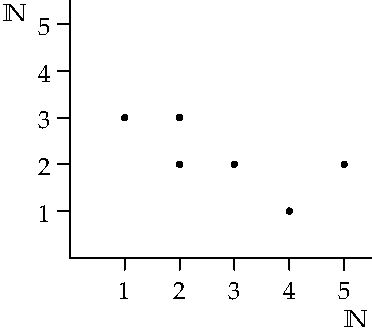
\includegraphics[width=\textwidth]{relations-01-reln1}\\
		Example 1.
	\end{minipage}\qquad\qquad\qquad
	\begin{minipage}{0.3\textwidth}\centering
		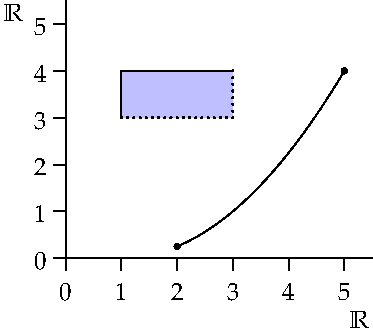
\includegraphics[width=\textwidth]{relations-02-reln2}\\
		Example 2.
	\end{minipage}
\end{center}
Not all relations between sets of numbers can be graphed: for example, graphing the relation $\cR=\Q\times\Q$ is impossible!\par


\begin{minipage}[t]{0.6\linewidth}\vspace{0pt}
	To refer to the introduction, the standard ordering $<$ on $\N$ is a relation, and we can graph it: for all $x,y\in\N$, we define
	\[
		x\,\cR\,y\iff x<y
	\]
	or equivalently,
	\[
		\cR=\{(x,y)\in\N\times\N:x<y\}
	\]
	\vspace*{10pt}
\end{minipage}
\hfill
\begin{minipage}[t]{0.35\linewidth}\vspace{0pt}
	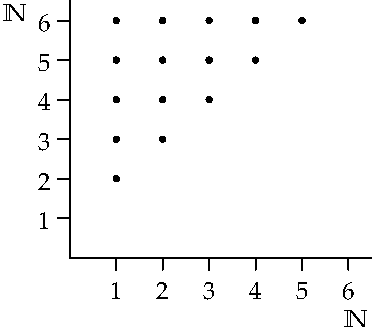
\includegraphics[width=\textwidth]{relations-25-less}
\end{minipage}\par

We can also think about functions in this language: if $f:\R\to\R$ is a function, then we could define
\[
	x\,\cR\,y\iff y=f(x)
\]
or equivalently
\[
	\cR=\{(x,y)\in\R^2:y=f(x)\}
\]
We will return to this viewpoint on function in the Section \ref{sec:func2}.


\boldsubsubsection{Basic results regarding relations}

With abstract relations, there are only a small number of things we can do.

\begin{defn}{}{relnsym}
	If $\cR\subseteq A\times B$ is a relation, then its \emph{inverse} $\cR^{-1}\subseteq B\times A$ is the set
	\[
		\cR^{-1}=\{(y,x)\in B\times A:(x,y)\in\cR\}
	\]
	To find the elements of $\cR^{-1}$, you simply switch the components of each ordered pair in $\cR$.\par
	Suppose $A=B$. We say that $\cR$ is \emph{symmetric} if $\cR=\cR^{-1}$.
\end{defn}

The following results should seem natural, even if some of the proofs may not be obvious.

\begin{thm}{}{relbasic}
	Given any relations $\cR,\cS\subseteq A\times B$:
	\begin{enumerate}
		\item $(\cR^{-1})^{-1}=\cR$
		\item $\cR\subseteq \cS\iff \cR^{-1}\subseteq \cS^{-1}$
		\item $(\cR\cup \cS)^{-1}=\cR^{-1}\cup \cS^{-1}$
		\item $(\cR\cap \cS)^{-1}=\cR^{-1}\cap \cS^{-1}$
		\item If $A=B$, then $\cR\cup \cR^{-1}$ is symmetric
		\item If $A=B$, then $\cR\cap \cR^{-1}$ is symmetric
	\end{enumerate}
\end{thm}

\begin{proof}
	Here are two of the arguments. Try the others yourself.
	\begin{enumerate}
		\item[2.] Assume that $\cR\subseteq\cS$, and suppose that $(x,y)\in\cR^{-1}$. We must prove that $(x,y)\in\cS^{-1}$. By the definition of inverse,
		\begin{align*}
			(x,y)\in\cR^{-1}&\implies (y,x)\in\cR\implies (y,x)\in\cS\\
			&\implies (x,y)\in\cS^{-1}
		\end{align*}
		Therefore $\cR^{-1}\subseteq\cS^{-1}$. For the converse, suppose that $\cR^{-1}\subseteq\cS^{-1}$. Then, by an argument similar to the above, we see that $(\cR^{-1})^{-1}\subseteq (\cS^{-1})^{-1}$. Now use 1.\ to see that
		\[
			\cR^{-1}\subseteq\cS^{-1}\implies\cR\subseteq \cS
		\]
		\item[5.] By 3,
		\[
			(\cR\cup \cR^{-1})^{-1}=\cR^{-1}\cup (\cR^{-1})^{-1}=\cR^{-1}\cup \cR=\cR\cup \cR^{-1}
		\]
		and so $\cR\cup \cR^{-1}$ is symmetric.\qedhere
	\end{enumerate}
\end{proof}

{\bf Keep your proof skills sharp!}\quad Several parts of Theorem \ref{thm:relbasic} look suspiciously similar to earlier results and it is easy to get confused. For example, 3 and 4 look almost like De Morgan's laws, except that $\cup$ and $\cap$ do not switch over. This is why it is important to be able to conjure up examples and \emph{prove} such statements. There are many facts in mathematics: trying to memorize everything is too difficult! Instead, you will be forever conjecturing and having to justify your guesses. For example, suppose that you forget results 3 and 4: it seems reasonable to conjecture that
\[
	(\cR\cup \cS)^{-1}=
	\begin{cases}
		\cR^{-1}\cup \cS^{-1}\\
		\qquad\text{or}\\
		\cR^{-1}\cap \cS^{-1}
	\end{cases}
\]
Now that you have two sensible guesses, you should be able to decide the correct one by thinking about examples and, if necessary, proving your assertion!

\begin{example}{}{}
	Consider Example 1 from before: $\cR=\{(1,3),(2,2),(2,3),(3,2),(4,1),(5,2)\}\subseteq\N\times\N$. This is not symmetric since, for example, $1\,\cR\,3$ but $3\not\!\!\cR\,1$. We compute
	\[
		\cR^{-1}=\{(3,1),(2,2),(3,2),(2,3),(1,4),(2,5)\},
	\]
	and observe that
	\begin{gather*}
		\cR\cap \cR^{-1}=\{(2,2), (2,3), (3,2)\}\quad\text{and}\quad \\
		\cR\cup \cR^{-1}=\{(1,3),(3,1),(2,2),(2,3),(3,2),(4,1),(1,4),(5,2),(2,5)\}
	\end{gather*}
	are both symmetric.
\end{example}

\begin{center}
	\begin{minipage}{0.35\textwidth}\centering
		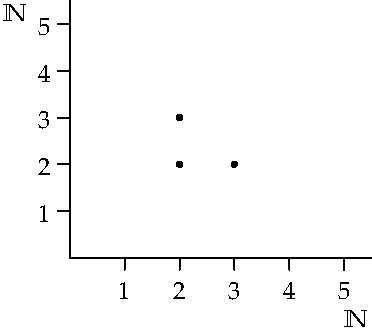
\includegraphics[width=\textwidth]{relations-03-relnint}\\
		The relation $\cR\cap \cR^{-1}$
	\end{minipage}
	\qquad\qquad\qquad
	\begin{minipage}{0.35\textwidth}\centering
		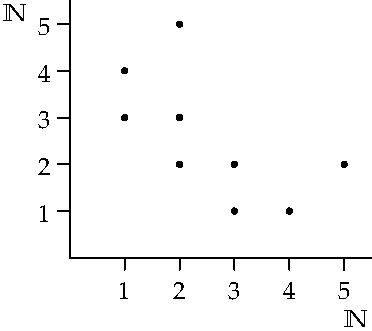
\includegraphics[width=\textwidth]{relations-04-relnun}\\
		The relation $\cR\cup \cR^{-1}$
	\end{minipage}
\end{center}

These pictures should confirm something intuitive: if you are able to graph a symmetric relation, then the graph will have symmetry about the line $y=x$. Indeed, $\cR^{-1}$ is obtained by reflecting $\cR$ in the line $y=x$. Recall how to graph an inverse functions from calculus\ldots

% \paragraph{Self-test Questions}
% 
% 	\begin{enumerate}
%     \item A \emph{relation} $\cR$ from a set $A$ to a set $B$ is \underline{\phantom{a subset of $A\times B$}\qquad\qquad} 
%     \item If $A\subseteq\R$, then the graph of a symmetric relation $\cR\subseteq A\times A$ has what sort of symmetry?
%     \item True or false: if $\cR$ is symmetric, then it must contain an even number of elements.
%   \end{enumerate}

\begin{exercises}{}{}
\begin{enumerate}
  \item Let $\cR$ be the relation on $\{0,1,2\}$ defined by
  \[0\,\cR\,0\qquad 0\,\cR\,1\qquad 2\,\cR\,1\]
  \begin{enumerate}
    \item Write $\cR$ as a set of ordered pairs.
    \item What is the inverse of $\cR$?
	\end{enumerate}
	
	\item Let $\cR$ be the relation on $\R$ defined by $x\,\cR\,y\iff\nm{x-y}=1$. Draw $\cR$. Is it symmetric?
  
	\item Draw pictures of the following relations on the set of real numbers $\R$.
		\begin{enumerate}
			\item $\cR=\{(x,y):y\le x\text{ and }y\le 2\text{ and }y\le 2-x\}$.
			\item $\cS=\{(x,y):(x-4)^2+(y-1)^2\le 9\}$.
		\end{enumerate}
	Also draw the inverse of each relation.
	
	\item A relation is defined on $\N$ by $a\,\cR\,b\!\iff\! \frac ab\in\N$. Let $c,d\in\N$. Under what conditions is it permissable to write $c\,\cR^{-1}\,d$?
	
	\item Let $\cR\subseteq\{1,2,3,4\}\times\{1,2,3,4\}$ be the relation
	\[\cR=\{(1,3),(1,4),(2,2),(2,4),(3,1),(3,2),(4,4)\}.\]
	\begin{enumerate}
	  \item Compute $\cR^{-1}$.
	  \item Compute the relations $\cR\cup \cR^{-1}$ and $\cR\cap \cR^{-1}$, and check that they are symmetric.
	\end{enumerate}
  
  \item For the relation $\cR=\{(x,y):x\le y\}$ defined on $\N$, what is $\cR^{-1}$, and what is the intersection $\cR\cap\cR^{-1}$?

  \item Let $A$ be a set with $\nm A=4$. What is the maximum number of elements that a relation $\cR$ on $A$ can contain such that $\cR\cap \cR^{-1}=\emptyset$?
  
  \item Give formal proofs of the remaining cases (1, 3, 4 \& 6) of Theorem \ref{thm:relbasic}.
  
  \item Let $\cR$ be a relation on a set $A$ and define $\cS=\cR\cup\cR^{-1}$. We know that $\cS$ is symmetric. Prove that $\cS$ is the intersection of all \emph{symmetric} relations on $A$ which contain $\cR$. Otherwise said: if
  \[\mathrm T=\Bigl\{\mathcal T\subseteq A\times A:\mathcal T\text{ symmetric and }\cR\subseteq\mathcal T\bigr\}\]
  then
  \[\cS=\bigcap\limits_{\mathcal T\in \mathrm T} \mathcal T\]
  \emph{$\cS$ is known as the \emph{symmetric closure} of $\cR$.}
\end{enumerate}

\end{exercises}

\clearpage


\subsection{Functions revisited}\label{sec:func2}

Now that we have the language of relations, we can properly define functions. Recall that a function $f:A\to B$ is a rule that assigns one, and only one, element of $B$ to each element of $A$. We may therefore view $f$ as a collection of ordered pairs in $A\times B$:
\[
	\big\{(a,f(a)):a\in A\big\}
\]
This set is nothing more than the \emph{graph} of the function, and, being a set of ordered pairs, it is a relation.

\begin{defn}{}{func}
	Let $\cR\subseteq A\times B$ be a relation from $A$ to $B$. The \emph{domain} and \emph{range} of $\cR$ are the sets
	\begin{gather*}
		\dom(\cR)=\{a\in A:(a,b)\in \cR\text{ for some }b\in B\},\\
		\range(\cR)=\{b\in B:(a,b)\in \cR\text{ for some }a\in A\}.
	\end{gather*}
	A \emph{function} from $A$ to $B$ is a relation $f\subseteq A\times B$ satisfying the following conditions:
	\begin{enumerate}
	  \item $\dom(f)=A$,
	  \item $(a,b_1),(a,b_2)\in f\implies b_1=b_2$.
	\end{enumerate}
\end{defn}

The two conditions can be thought of as saying:
\begin{enumerate}
  \item Every element of $A$ is related to \emph{at least one} element of $B$.
  \item Every element of $A$ is related to \emph{at most one} element of $B$.
\end{enumerate}
Putting these together, we see that a relation $f\subseteq A\times B$ is a function if \emph{every} $a\in A$ is the first entry of one (and only one) ordered pair $(a,b)\in f$. The second condition is the vertical line test, familiar from calculus.

\begin{center}
	\begin{minipage}{0.32\textwidth}\centering
		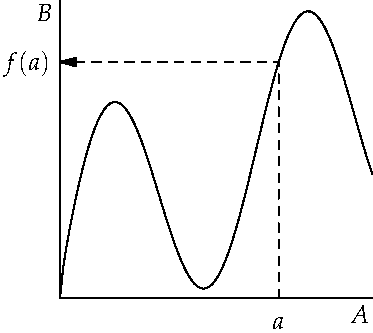
\includegraphics[width=\textwidth]{relations-05-funcvert}\\
		$b_1=b_2=f(a)$: a function
	\end{minipage}\qquad\qquad\qquad\qquad
	\begin{minipage}{0.32\textwidth}\centering
		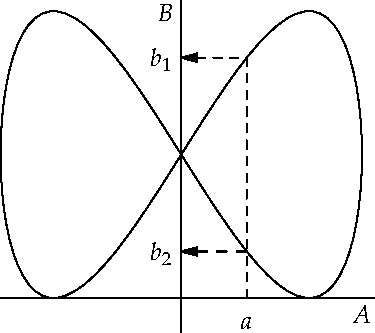
\includegraphics[width=\textwidth]{relations-06-funcvert}\\
		$b_1\neq b_2$: not a function
	\end{minipage}
\end{center}

We can also think about injectivity and surjectivity (recall Definition \ref{defn:11}) in this context. A function $f\subseteq A\times B$ is:
\begin{itemize}
  \item \emph{Injective} if no two pairs in $f$ share the same second entry.
  \item \emph{Surjective} if every $b\in B$ appears as the second entry of at least one pair in $f$.
  \item \emph{Bijective} if every $b\in B$ appears as the second entry of one (and only one) ordered pair $(a,b)\in f$.
\end{itemize}


\begin{example}{}{}
	Let $A=B=\{1,2,3\}$ and consider the relation\par
	\begin{minipage}[t]{0.62\linewidth}\vspace{0pt}
		\[
			f=\{(1,3),(2,1),(3,3)\}
		\]
		Observe that $\dom(f)=\{1,2,3\}=A$, and that each element of $A$ appears exactly once as the first element in a pair $(a,b)\in f$. The relation therefore satisfies both conditions necessary to be a function. In more elementary language we would write $f(1)=3$, \ $f(2)=1$ and $f(3)=3$.\par
		Since 3 appears twice as a second entry of an ordered pair in $f$ we see that $f$ is \emph{not injective.}\par
		Since 2 never appears as the second entry of an ordered pair in $f$ we see that $f$ is \emph{not surjective.}
	\end{minipage}
	\hfill
	\begin{minipage}[t]{0.35\linewidth}\vspace{0pt}
		\centering
		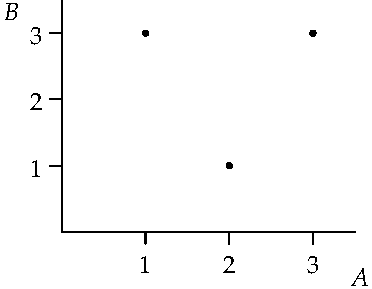
\includegraphics[scale=0.8]{relations-18-reln1}\\
		A function $f:A\to B$
	\end{minipage}
\end{example}

\boldsubsubsection{The Inverse of a Function}

Since every function is a relation, it is a straightforward business to define the inverse of a function.

\begin{defn}{}{}
	The \emph{inverse} of a function $f\subseteq A\times B$ is the inverse relation $f^{-1}\subseteq B\times A$.
\end{defn}

To compute an inverse relation we simply reverse the components of each ordered pair: the following should therefore be clear.

\begin{thm}{}{inversedomrange}
	$\dom(f^{-1})=\range(f)$ \ and \ $\range(f^{-1})=\dom(f)$
\end{thm}

In general, you should expect the inverse of a function to be merely a relation and not a function in its own right. We shall shortly (Theorem \ref{thm:finverse}) discuss when the inverse relation is a function.

\begin{example*}{cont}{}
	Consider the above example.\par
	\begin{minipage}[t]{0.62\linewidth}\vspace{0pt}
		The inverse relation
		\[
			f^{-1}=\{(3,1),(1,2),(3,3)\}\subseteq B\times A
		\]
		is \emph{not} a function due to failing \emph{both} conditions of Definition \ref{defn:func}.
		\begin{itemize}
		  \item $\dom(f^{-1})=\{1,3\}$ is not the whole of $B$.
		  \item $(3,1)\in f^{-1}$ and $(3,3)\in f^{-1}$, but $1\neq 3$.
		\end{itemize}
		Both failures are clearly visible in the picture.
	\end{minipage}
	\hfill
	\begin{minipage}[t]{0.33\linewidth}\vspace{0pt}
		\centering
		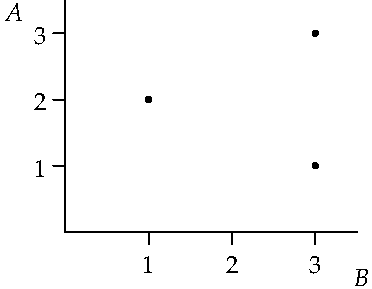
\includegraphics[width=\textwidth]{relations-19-reln1}\\
		$f^{-1}\subseteq B\times A$: not a function
	\end{minipage}
\end{example*}

Before we consider exactly when the inverse of a function is a function in its own right, we consider a few more examples.


\begin{examples}{}{}
	\begin{enumerate}
		\item\label{ex:reln1} Let $A=B=\R$ and $f=\{(x,x^2):x\in\R\}$. This is simply the function with formula $f(x)=x^2$. The inverse relation $f^{-1}\subseteq\R\times\R$ is then
		\[
			f^{-1}=\bigl\{(x^2,x):x\in\R\bigr\}=\bigl\{(y,\pm\sqrt y):y\ge 0\bigr\}
		\]
		In this case, $f^{-1}$ is \emph{not a function.} In the language of Definition \ref{defn:func}:
		\begin{itemize}
		  \item $\dom(f^{-1})=\R^+_0\neq B$. E.g., $-1\in B$ but $-1\not\in\dom(f^{-1})$.
		  \item $(4,2)$ and $(4,-2)$ are distinct elements of $f^{-1}$ with the same first entry.
		\end{itemize}
		\begin{center}
			\begin{minipage}{0.35\textwidth}\centering
				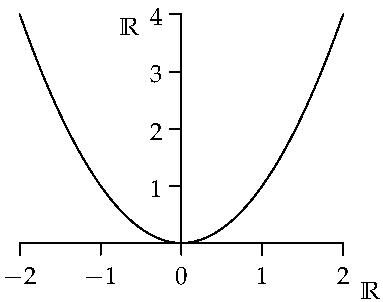
\includegraphics[width=\textwidth]{relations-20-reln2}\\
				$f:A\to B$
			\end{minipage}\qquad\qquad\qquad
			\begin{minipage}{0.35\textwidth}\centering
				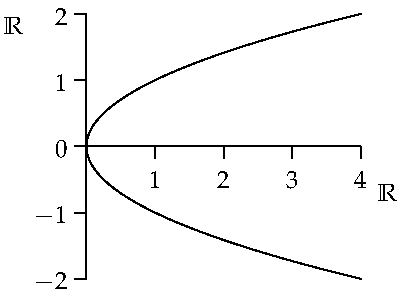
\includegraphics[width=\textwidth]{relations-21-reln2}\\
				$f^{-1}\subseteq B\times A$: not a function
			\end{minipage}
		\end{center}
		It should be obvious that $f$ is neither injective nor surjective: in the language of relations,
		\begin{description}
			\item[Not injective]\quad $(2,4)$ and $(-2,4)$ are distinct elements of $f$ with the same second entry.
			\item[Not surjective]\quad For instance, $-1$ never appears as the second entry of any pair in $f$.
		\end{description}
		Observe how these are merely a rewriting of what it means for $f^{-1}$ to fail to be a function.
		
		\item\label{ex:reln2} Let $A=B=\R$ and $f=\{(x,x^3):x\in\R\}$, so that $f$ has formula $f(x)=x^3$. This time, the inverse is also a function and we could write $f^{-1}(y)=\sqrt[3]{y}$:
		\[
			f^{-1}=\bigl\{(x^3,x):x\in\R\bigr\}=\bigl\{(y,\sqrt[3]{y}):y\in\R\bigr\}
		\]
		\begin{center}
			\begin{minipage}{0.35\textwidth}\centering
				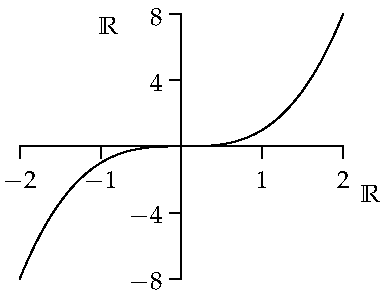
\includegraphics[width=\textwidth]{relations-22-reln3}\\
				$f:A\to B$
			\end{minipage}\qquad\qquad\qquad
			\begin{minipage}{0.35\textwidth}\centering
				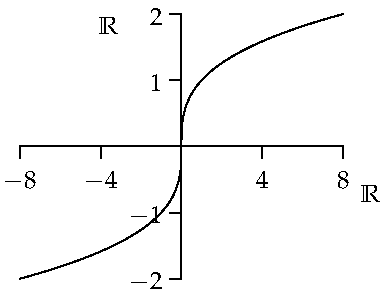
\includegraphics[width=\textwidth]{relations-23-reln3}\\
				$f^{-1}:B\to A$ is a function
			\end{minipage}
		\end{center}
	\end{enumerate}
\end{examples}

All three of our examples help to illustrate the following important result.

\begin{thm}{}{finverse}
	A relation $f^{-1}\subseteq B\times A$ is a function $\iff f$ is bijective (both injective and surjective).
\end{thm}

\begin{proof}
	Recalling Definition \ref{defn:func}, we see that
	\[
		f^{-1}\text{ is a function }\iff
		\begin{cases}
			\dom(f^{-1})=B,\\
			\qquad\text{\emph{and}}\\
			(b,a_1),(b,a_2)\in f^{-1}\implies a_1=a_2.
		\end{cases}
	\]
	The first of these is equivalent to $\range(f)=B$, which says that $f$ is surjective.\par
	The second is equivalent to $(a_1,b),(a_2,b)\in f\implies a_1=a_2$, which says that $f$ is injective.
\end{proof}

Here is a final example, where the function $f$ is harder to visualize.

\begin{example}{}{}
	Let $A=\R$, $B=\Q$ and define $f$ using the formula 
	\[
		f(x)=
		\begin{cases}
			x&\text{if }x\in\Q,\\
			0&\text{if }x\not\in\Q.
		\end{cases}
	\]
	In the language of relations, this is $f=\bigl\{(x,x):x\in\Q\bigr\}\cup\bigl\{(x,0):x\not\in\Q\bigr\}$.\par
	This is a surjective function since every element of $B=\Q$ appears as the second entry in an ordered pair $(a,b)\in f$. It is not injective since zero appears more than once in the second entry. For example,
	\[
		(\sqrt 2,0),\ (\sqrt 3,0)\in f
	\]
	Written in the more common manner, we are observing that $f(\sqrt 3)=f(\sqrt 2)$.\par
	The inverse $f^{-1}$ is not a function, and it fails to be so precisely because $f$ is non-injective. For example
	\[
		(0,\sqrt 2)\text{ and } (0,\sqrt 3)\text{ are distinct elements of $f^{-1}$ with the same  first component.}
	\]
\end{example}

\boldinline{Inverse Images}

Analogously to the concept of images of sets (Section \ref{sec:func1}), we can define the \emph{inverse image} of a subset $V\subseteq B$ under a function $f:A\to B$ by
\[
	f^{-1}(V)=\{a\in A:f(a)\in V\}
\]
In particular, if $\{b\}\subseteq B$ has only one element, then its inverse image is
\[
	f^{-1}(\{b\})=\{a\in A:f(a)=b\}
\]
Both are \emph{subsets} of $A$. For instance, in the last example the inverse image of $\{0\}$ consists of zero and all irrational numbers!
\[
	f^{-1}(\{0\})=\{0\}\cup(\R\setminus\Q)
\]
When $f^{-1}\subseteq B\times A$ is a function, each inverse image of a singleton consists of one point of $A$: thus $f^{-1}(\{b\})=\{a\}$. \emph{Only} in such a case are we entitled to write $f^{-1}(b)=a$.




\begin{aside}{}{}
{\bf Equality of functions}

There are two competing notions of what it means for two functions to be \emph{equal.}

\begin{description}
	\item[Same domain, same graph, same codomain]\quad $f=g$ means that $f$ and $g$ are the same subset of the \emph{same} $A\times B$. This notion is preferred by set theorists because it sticks rigidly to the idea that a function is a \emph{relation,} and it requires both the domain $A$ and codomain $B$ to be explicit.
	\item[Same domain, same graph]\quad $f=g$ means that $f\subseteq A\times B$, \ $g\subseteq A\times C$, and
	\[(a,b)\in f\iff (a,b)\in g.\]
	This notion considers what a function \emph{does} to be fundamental; if two functions do the same thing to elements of the same domain then they are the same. This looser notion of equality is used more often, especially in elementary calculus.
\end{description}

The second conception of equality, while intuitive, has a problem. For example, let
\[
	f:\R\to\R,\quad\text{and}\quad g:\R\to[-1,1]\quad\text{satisfy}\quad f(x)=g(x)=\sin x
\]
Although $f$ and $g$ have the same graph, the different codomains of $f$ and $g$ mean that these are \emph{different functions} with respect to the first notion. Under the second notion, they are the \emph{same function.} However, $g$ is surjective while $f$ is not, so wouldn't we prefer $f$ and $g$ to be non-equal?\footnote{In elementary calculus, we usually say that a function is invertible if it is 1--1. In order for this to make sense, we have to ignore surjectivity and use the second notion of functional equality.}\par


The same problem does not arise when considering domains. For example, in calculus you might have compared functions such as
\[
	f(x)=x^2+2,\quad\text{and}\quad g(x)=\frac{(x^2+2)(x-1)}{x-1}
\]
The implied domains of these functions are $\dom(f)=\R$ and $\dom(g)=\R\setminus\{1\}$. Even though these have the same graph whenever \emph{both} are defined, regardless of which notion you choose we have $f\neq g$, since the functions have \emph{different domains.}
\end{aside}
% 
% \paragraph{Self-test Questions}
% 
% 	\begin{enumerate}
%     \item What does it mean for a \emph{relation} $\cR\subseteq A\times B$ to be a \emph{function}?
%     \item If $f\subseteq A\times B$ is a function, what does it mean, in the language of relations, for $f$ to be \emph{injective}? \emph{Surjective}?
%     \item True or false: a relation $\cR$ has a domain and range if and only if it is a function.
%   \end{enumerate}


\begin{exercises}{}{}

\begin{enumerate}
  \item Suppose that $f\subseteq\{1,2,3,4\}\times\{1,2,3,4,5,6,7\}$ is the relation
  \[f=\{(1,1),(2,3),(3,5),(4,7)\}.\]
  \begin{enumerate}
    \item Show that $f$ is a function $f:\{1,2,3,4\}\to\{1,2,3,4,5,6,7\}$. Can you find a concise formula $f(x)$ to describe $f$?
    \item Is $f$ injective? Justify your answer.
    \item Suppose that $g\subseteq\{1,2,3,4\}\times B$ is another relation so that the \emph{graphs} of $f$ and $g$ are identical: i.e.
    \[\bigl\{(a,f(a)):a\in\{1,2,3,4\}\bigr\}=\bigl\{(a,g(a)):a\in\{1,2,3,4\}\bigr\}.\] \emph{as sets.} If $g$ is a bijective function, what is $B$?
  \end{enumerate}
  
  \item Decide whether each of the following relations are functions. For those which are, decide whether the function is injective and/or surjective.
  \begin{enumerate}
    \item $\cR=\{(x,y)\in[-1,1]\times[-1,1]:x^2+y^2=1\}$
    \item $\cS=\{(x,y)\in[-1,1]\times[0,1]:x^2+y^2=1\}$
    \item $\mathcal T=\{(x,y)\in[0,1]\times[-1,1]:x^2+y^2=1\}$
    \item $\mathcal U=\{(x,y)\in[0,1]\times[0,1]:x^2+y^2=1\}$
  \end{enumerate}
  
  \item In Example \ref{ex:reln2} on page \pageref{ex:reln2}, explain why the function $f$ is both injective and surjective using the language of relations: i.e., in the same manner as we analyzed Example \ref{ex:reln1}.
  
  \item For each of the examples on page \pageref{ex:reln2}, compute the following inverse images:
  \begin{enumerate}
    \item $f^{-1}(\{0,1\})$
    \item $f^{-1}\Big([0,1)\Big)$
    \item $f^{-1}\Big((-\infty,0]\Big)$
    \item $f^{-1}\Big(\{-8\}\cup[-7,2]\cup (3,9)\Big)$
  \end{enumerate}
  
  \item\begin{enumerate}
    \item Express the function $f:\R\to\R:x\mapsto x^4+3$ as a relation.
    \item What is the inverse relation $f^{-1}$?
    \item Use Definition \ref{defn:func} to prove that the relation $f^{-1}$ is \emph{not} a function.
    \item Prove directly from Definition \ref{defn:11} that $f$ is not injective and not surjective. Compare your arguments with your answer to part (c).
  \end{enumerate}
  
  \item Repeat the previous question for $f:\R\to\R:x\mapsto \sqrt{x^2-4x+5}$.
  
  \item Give a formal proof of Theorem \ref{thm:inversedomrange}.
  
  \item Prove or disprove the following: if $f:A\to B$ is a function, and $U,V\subseteq B$, then
  \[f^{-1}(U\cap V)=f^{-1}(U)\cap f^{-1}(V)\]
\end{enumerate}

\end{exercises}

\clearpage



\subsection{Equivalence Relations}\label{sec:equiv}

In mathematics, the notion of \emph{equality} is not as simple as one might think. The idea of two numbers being equal is straightforward, but suppose we want to consider two paths between given points as `equal' if and only if they have the same length? Since two `equal' paths might look very different, is this a good notion of equality? Mathematicians often want to gather together objects that have a common property and then treat them as if they were a single object. This is done using equivalence relations and equivalence classes.\par

First recall the alternative notation for a relation on a set $A$: if $\cR\subseteq A\times A$ is a relation on $A$, then $x\,\cR\,y$ has the same meaning as $(x,y)\in\cR$. We might read $x\,\cR\,y$ as `$x$ is $\cR$-related to $y$.'

\newsavebox\mybox
\sbox{\mybox}{\emph{Transitivity}}
\def\refl{\makebox[\wd\mybox][l]{\emph{Reflexivity}}}
\def\symm{\makebox[\wd\mybox][l]{\emph{Symmetry}}}
\def\trans{\makebox[\wd\mybox][l]{\emph{Transitivity}}}

\begin{defn}{}{}
A relation $\cR$ on a set $A$ may be described as \emph{reflexive, symmetric} or \emph{transitive} if it satisfies the following properties:
\begin{itemize}
  \item \refl $\forall x\in A$, \ $x\,\cR\,x$\hfill(every element of $A$ is related to itself)
  \item	\symm $\forall x,y\in A,\ x\,\cR\,y\implies y\,R\,x$\hfill(if $x$ is related to $y$, then $y$ is related to $x$)
  \item	\trans $\forall x,y,z\in A,\ x\,\cR\,y$ \ and \ $y\,\cR\,z\implies x\,\cR\,z$\hfill(if $x$ is related to $y$, and $y$ is related to $z$, \phantom{bob}\hfill then $x$ is related to $z$)
	\end{itemize}
\end{defn}

Symmetry is exactly the same notion as in Definition \ref{defn:relnsym}.

\begin{examples}{}{}
	\begin{enumerate}
	\item Let $A=\R$ and let $\cR$ be $\le$. Thus $2\le 3$, but $7\nleq 4$. We check whether $\cR$ satisfies the above properties.
	\begin{itemize}
		\item \refl True. $\forall x\in\R$, \ $x\le x$.
		\item \symm False. For example, $2\le 3$ but $3\nleq 2$.
		\item \trans True. $\forall x,y,z\in\R$, if $x\le y$ and $y\le z$, then $x\le z$.
	\end{itemize}
	\item Let $A$ be the set of lines in the plane and define $\ell_1\,R\,\ell_2\iff \ell_1$ and $\ell_2$ intersect.\par
	\begin{minipage}[t]{0.65\linewidth}\vspace{0pt}
		\begin{itemize}
			\item \refl True. Every line intersects itself, so $\ell\,\cR\,\ell$ for all $\ell\in A$.
			\item \symm True. For all lines $\ell_1,\ell_2\in A$, if $\ell_1$ intersects $\ell_2$, then $\ell_2$ intersects $\ell_1$.
			\item \trans False. As the picture illustrates, we may let $\ell_1$ and $\ell_3$ be parallel lines, and $\ell_2$ cross both of these. Then $\ell_1\,\cR\,\ell_2$ and $\ell_2\,\cR\,\ell_3$, but $\ell_1\not\!\!\cR\,\ell_3$.
		\end{itemize}
	\end{minipage}
	\hfill
	\begin{minipage}[t]{0.3\linewidth}\vspace{0pt}
		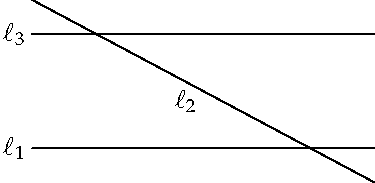
\includegraphics[width=\textwidth]{relations-07-parallel}
	\end{minipage}
\end{enumerate}
\end{examples}

\begin{defn}{}{}
	An \emph{equivalence relation} is a relation $\sim$ which is reflexive, symmetric and transitive.
\end{defn}

The symbol $\sim$ is almost universally used for an abstract equivalence relation. It can be read as `related to,' `tilde,' or `twiddles.' The two examples above are \emph{not} equivalence relations because they fail one of the three conditions. We now exhibit the simplest equivalence relation.

\begin{example}{}{}
	Equals `=' is an equivalence relation on any set, hence the name!
\end{example}

Read the definitions of reflexive, symmetric and transitive until you are certain of this fact. There are countless other equivalence relations: here are a few.

\begin{examples}{}{}
\begin{enumerate}
	\item For all $x,y\in\Z$, we define the relation $\sim$ by
	\[
		x\sim y\iff x-y\ \text{ is even.}
	\]
	We claim that $\sim$ is an equivalence relation on $\Z$.
	\begin{itemize}
		\item \refl $\forall x\in\Z,\ x-x=0$ is even, hence $x\sim x$.
		\item \symm $\forall x,y\in\Z,\ x\sim y\implies x-y$ is even $\implies y-x$ is even $\implies y\sim x$.
		\item \trans$\forall x,y,z\in\Z$, if $x\sim y$ and $y\sim z$, then $x-y$ and $y-z$ are even. But the sum of two even numbers is even, hence $x-z=(x-y)+(y-z)$ is even, and so $x\sim z$.
	\end{itemize}
	
	\item Let $A=\{$all students taking this course$\}$. For all $x,y\in A$, let
	\[x\sim y\iff x\ \text{ achieves the same letter-grade as $y$.}\]
	Then $\sim$ is an equivalence relation on $A$; here is the proof.
	\begin{itemize}
		\item \refl $\forall x\in A,\ x\sim x$ since everyone scores the same as themself!
		\item \symm $\begin{array}[t]{@{}rl}
			\forall x,y\in A,\ x\sim y&\implies x\ \text{achieves the same letter-grade as $y$}\\
			&\implies y\ \text{achieves the same letter-grade as $x$}\\
			&\implies y\sim x
		\end{array}$
		\item \trans$\forall x,y,z\in A$, if $x\sim y$ and $y\sim z$, then $x$ achieves the same as $y$ who achieves the same as $z$, whence $x$ achieves the same as $z$. Thus $x\sim z$.
	\end{itemize}

	\item We define an equivalence relation on $\Z$ by
	\[
		\forall x,y\in\Z,\ \ x\sim y\iff x^2\equiv y^2\pmod 5
	\]
		\begin{itemize}
			\item \refl $\forall x\in\Z,\ x\sim x$ since $x^2$ is always congruent to itself!
			\item \symm $\begin{array}[t]{@{}rl}
				\forall x,y\in\Z,\ x\sim y&\implies x^2\equiv y^2\pmod 5\\
				&\implies y^2\equiv x^2\pmod 5\\
				&\implies y\sim x
			\end{array}$
			\item \trans $\forall x,y,z\in\Z$, if $x\sim y$ and $y\sim z$, then $x^2\equiv y^2$ and $y^2\equiv z^2\pmod 5$. But then $x^2\equiv z^2\pmod 5$ and so $x\sim z$.
	\end{itemize}
\end{enumerate}
\end{examples}

The most important thing to observe in each of these examples is that {\bf an equivalence relation separates elements of a set into subsets where elements share a common property} (even/oddness, letter-grade, etc.). The next definition formalizes this idea.

\begin{defn}{}{equivrel}
	Let $\sim$ be an equivalence relation on a set $X$. The \emph{equivalence class} of an element $x\in X$ is the set
	\[
		[x]=\{y\in X:y\sim x\}
	\]
	Otherwise said, $y\sim x\iff y\in[x]$. The set of all equivalence classes is known as the \emph{quotient} of $X$ by $\sim$ or simply `$X$ mod $\sim$,' and is denoted
	\[
		\quotient X\sim=\Big\{[x]:x\in X\Big\}
	\]
\end{defn}

Let us think about the definition of equivalence class in the context of our previous examples.

\begin{examples}{}{}
	\begin{enumerate}
		\item $[0]=\{y\in\Z:y\sim 0\}=\{y\in\Z:y\text{ is even}\}$ is the set of even numbers. Note that $[0]=[2]=[4]=[6]$, etc. The other equivalence class is $[1]=\{y\in\Z:y-1\text{ is even}\}$, which is the set of odd numbers. The quotient set is
		\[
			\smash{\quotient \Z\sim}=\bigl\{[0],[1]\bigr\}=\bigl\{\{\text{even numbers}\},\{\text{odd numbers}\}\bigr\}
		\]
	
		\item There is one equivalence class for each letter grade awarded. Each equivalence class contains all the students who obtain a particular letter-grade. If we call the equivalence classes $\mathrm{A^+,A,A^-,B^+,\ldots,F}$, where, say, $\mathrm B=\{$students obtaining a B-grade$\}$, then
		\[
			\smash{\quotient{\{\text{Students}\}}{\sim}}=\{\mathrm{A^+,A,A^-,B^+,\ldots,F}\}
		\]
	
		\item The equivalence classes for this example are a little tricky. First observe that
		\[
			x\equiv y\spmod 5\implies x^2\equiv y^2\spmod 5
		\]
		so that there are at most five equivalence classes; those of 0, 1, 2, 3 and 4. Are they distinct?	If we square each of these and consider the remainder modulo 5, we obtain
		\[
			\begin{array}{l@{}r|c|c|c|c|c}
				x&\spmod 5&0&1&2&3&4\\\hline
				x^2&\spmod 5&0&1&4&4&1
			\end{array}
		\]
		Notice that $1\sim 4$, so they share an equivalence class. Similarly $2\sim 3$. Indeed the distinct equivalence classes are
		\begin{gather*}
			[0]=\{x\in\Z:x\equiv 0\spmod 5\}\\
			[1]=\{x\in\Z:x\equiv 1,4\spmod 5\}\\
			[2]=\{x\in\Z:x\equiv 2,3\spmod 5\}
		\end{gather*}
		In this case the quotient is the set
		\[
			\smash{\quotient{\Z}{\sim}}=\Bigl\{[0],[1],[2]\Bigr\}
		\]
	\end{enumerate}
\end{examples}

Here is one further example of an equivalence relation, this time on $\R^2$. Be careful with the notation: $\R^2=\R\times\R$ is already a Cartesian product, so a relation on $\R^2$ is a subset of $\R^2\times\R^2$!


\begin{example}{}{equivcircle}
Let $\sim$ be the relation on $\R^2$ defined by $(x,y)\sim(v,w)\iff x^2+y^2=v^2+w^2$. We claim that this is an equivalence relation.
	\begin{itemize}
		\item \refl $\forall (x,y)\in\R^2,\ x^2+y^2=x^2+y^2$.
		\item \symm $\begin{array}[t]{@{}rl}
		\forall (x,y),(v,w)\in\R^2,\ (x,y)\sim(v,w)&\implies x^2+y^2=v^2+w^2\\
		&\implies v^2+w^2=x^2+y^2\\
		&\implies (v,w)\sim(x,y)
		\end{array}$
		\item \trans $\forall (x,y),(v,w),(p,q)\in\R^2$, if $(x,y)\sim (v,w)$ and $(v,w)\sim (p,q)$, then $x^2+y^2=v^2+w^2$ and $v^2+w^2=p^2+q^2$. But then $x^2+y^2=p^2+q^2$ and so $(x,y)\sim (p,q)$.
	\end{itemize}
	
	$\sim$ is therefore an equivalence relation. But what are the equivalence classes? By definition,
	\[
		[(x,y)]=\Bigl\{(v,w)\in\R^2:v^2+w^2=x^2+y^2\Bigr\}
	\]
	\begin{minipage}[t]{0.6\linewidth}\vspace{0pt}
		This isn't particularly helpful. Indeed it is easier to think of each of these sets as
		\[
			\Bigl\{(v,w)\in\R^2:v^2+w^2\text{ is \emph{constant}}\Bigr\}
		\]
		Each equivalence class is therefore a \emph{circle} centered at the origin! Some of the equivalence classes are drawn in the picture: the class $[(1,0)]$ is highlighted. Moreover, the quotient set is
		\[
			\quotient{\R^2}{\sim}=\{\text{circles centered at the origin}\}
		\]
	\end{minipage}
	\hfill
	\begin{minipage}[t]{0.35\linewidth}\vspace{0pt}
		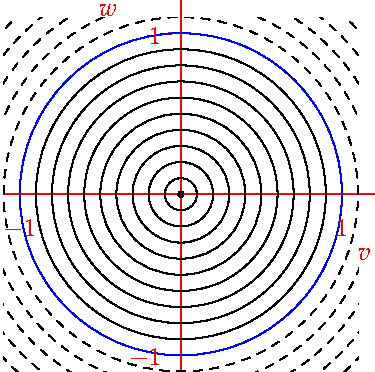
\includegraphics[width=\textwidth]{relations-24-circles}
	\end{minipage}
\end{example}

% \paragraph{Self-test Questions}
% 
% 	\begin{enumerate}
%     \item True or false: a relation $\sim$ on a set $X$ is \emph{reflexive} if $\exists x\in X$ such that $x\sim x$.
%    	\item An \emph{equivalence relation} satisfies which three properties? What do they mean?
%     \item Suppose that $x,y,z\in X$ and $\sim$ is an equivalence relation on $X$. Express each of the following assertions in terms of the properties satisfied by an equivalence relation.
%     \begin{enumerate}
%       \item $x\in[y]$ and $y\in[z]\implies x\in[z]$.
%       \item $x\in[x]$.
%       \item $x\in[y]\iff y\in[x]$.
%   	\end{enumerate}
%   \end{enumerate}

\begin{exercises}{}{}

\begin{enumerate}
	\item A relation $\cR$ is \emph{antisymmetric} if $((x,y)\in \cR)\wedge((y,x)\in \cR)\implies x=y$. Give examples of relations $\cR$ on $A=\{1,2,3\}$ having the stated property.
	\begin{enumerate}
		\item $\cR$ is both symmetric and antisymmetric.
		\item $\cR$ is neither symmetric nor antisymmetric.
		\item $\cR$ is transitive but $\cR\cup \cR^{-1}$ is not transitive.
	\end{enumerate}
	
	\item Let $\cS=\{(x,y)\in\R^2:\sin^2x+\cos^2y=1\}$.
	\begin{enumerate}
	  \item Give an example of two real numbers $x,y$ such that $x\,\cS\,y$.
	  \item Is $\cS$ reflexive? Symmetric? Transitive? Justify your answers.
	\end{enumerate}

	\item Each of the following relations $\sim$ is an equivalence relation on $\R^2$. Identify the equivalence classes and draw several of them.
	\begin{enumerate}
		\item $(a,b)\sim(c,d)\iff ab=cd$.
	  \item $(v,w)\sim(x,y)\iff v^2w=x^2y$.
	\end{enumerate}
	
  \item\begin{enumerate}
  \item Let $\sim$ be the relation defined on $\Z$ by $a\sim b\iff a+b$ is even. Show that $\sim$ is an equivalence relation and determine the distinct equivalence classes.
  \item Suppose that `even' is replaced by `odd' in part (a). Which of the properties reflexive, symmetric, transitive does $\sim$ possess?
  \end{enumerate}

  \item For each of the following relations $\cR$ on $\Z$, decide whether $\cR$ is reflexive, symmetric, or transitive, and whether $\cR$ is an equivalence relation.
	\begin{enumerate}
		\item $a\,\cR\,b \iff a\equiv b\pmod 3 \textbf{ or } a\equiv b\pmod 4$.
		\item $a\,\cR\,b \iff a\equiv b\pmod 3 \textbf{ and } a\equiv b\pmod 4$.
	\end{enumerate}

	\item For the purposes of this question, we call a real number $x$ \emph{small} if $\nm x\le 1$. Let $\cR$ be the relation on the set of real numbers defined by
	\[x\,\cR\,y \iff x-y \text{ is small}.\]
	\emph{Prove or disprove}: $\cR$ is an equivalence relation on $\R$.

	\item Let $A=\{1,2,3,4,5,6\}$. The distinct equivalence classes resulting from an equivalence relation $\sim$ on $A$ are $\{1,4,5\}$, $\{2,6\}$, and $\{3\}$. What is $\sim$? Give your answer as a subset of $A\times A$.

	\item $\subseteq$ is a relation on any set of sets. Is $\subseteq$ reflexive, symmetric, transitive? Prove your assertions.

	\item Let $S$ be the set of all polynomials of degree at most 3. An element $s\in S$ can then be expressed as
  \[s(x)=ax^3+bx^2+cx+d,\qquad\text{where $a,b,c,d\in\R$.}\]
  A relation $\cR$ on $S$ is defined by
  \[p\,\cR\,q\iff p\text{ and $q$ have a common root.}\]
  For example $p(x)=(x-1)^2$ and $q(x)=x^2-1$ have the root 1 in common so that $p\,\cR\,q$. Determine which of the properties reflexive, symmetric and transitive are possessed by $\cR$.

  \item Let $A=\{2^m:m\in\Z\}$. A relation $\sim$ is defined on the set $\Q^+$ of positive rational numbers by
  \[a\sim b\iff \frac ab\in A\]
  \begin{enumerate}
    \item Show that $\sim$ is an equivalence relation.
    \item Describe the elements in the equivalence class $[3]$.
  \end{enumerate}

  \item A relation is defined on the set $A=\{a+b\sqrt 2:a,b\in\Q,\,a+b\sqrt 2\neq 0\}$ by $x\sim y\iff \frac xy\in\Q$. Show that $\sim$ is an equivalence relation and determine the distinct equivalence classes.

	\item The \emph{reflexive, symmetric} and \emph{transitive closures} of a relation $\cR$ are defined respectively as the smallest relations containing $\cR$ which also exhibit the given property. Find each of the three closures of $\cR=\{(1,2),(2,3),(3,3)\}\subseteq\Z\times\Z$.

	\item Recall the description of the real projective line (page \pageref{ex:projline}): if $A_m$ is the line through the origin with gradient $m$, then
	\[\pr(\R^2)=\{A_m:m\in\R\cup\{\infty\}\}.\]
	Define a relation $\sim$ on $\R^2_*=\R^2\setminus\{(0,0)\}$ by $(a,b)\sim(c,d)\iff ad=bc$.
	\begin{enumerate}
	  \item Prove that $\sim$ is an equivalence relation.
	  \item Find the equivalence classes of $\sim$. How do the equivalence classes differ from the lines $A_m$?
	\end{enumerate}
  
	\item Suppose that $\cR,\cS$ are relations on some set $X$. Define the \emph{composition} $\cR\circ \cS$ to be the relation
	\[(a,c)\in \cR\circ \cS\iff \exists b\in X\text{ such that }(a,b)\in \cR\text{ and }(b,c)\in \cS.\]
	\begin{enumerate}
		\item If $\cR=\{(1,1),(1,2),(2,3),(3,1),(3,3)\}$ and $\cS=\{(1,2),(1,3),(2,1),(3,3)\}$, find $\cR\circ \cS$.
		\item Suppose that $\cR$ and $\cS$ are reflexive. Prove that $\cR\circ \cS$ is reflexive.
		\item Suppose that $\cR$ and $\cS$ are symmetric. Prove that $(x,y)\in \cR\circ \cS\iff (y,x)\in \cS\circ \cR$.
		\item Give an example of symmetric relations $\cR,\cS$ such that $\cR\circ \cS$ is \emph{not} symmetric. Conclude that if $\cR,\cS$ are equivalence relations, then $\cR\circ \cS$ need not be an equivalence relation.
	\end{enumerate}

  \item (\emph{Only for those who have studied Linear Algebra}) Let $\sim$ be the relation on the set of $2\times 2$ real matrices given by $A\sim B\iff\exists M$ such that $B=MAM^{-1}$.
  \begin{enumerate}
    \item Prove that $\sim$ is an equivalence relation.
    \item What is the equivalence class of the identity matrix?
    \item Show that $\left(\begin{smallmatrix}
    -11&15\\-5&9
    \end{smallmatrix}\right)\sim \left(\begin{smallmatrix}
    4&10\\0&-6
    \end{smallmatrix}\right)$ (\emph{Hint: think about diagonalizing})
    \item (Hard) Suppose that $L:\R^2\to\R^2$ is a linear map and $\beta,\gamma$ are bases of $\R^2$. Suppose that $A=[L]_\beta$ and $B=[L]_\gamma$ are the matrix representations of $L$ with respect to the two bases. Prove that $A\sim B$.
    \item (Hard) Suppose that $A,B$ have the same, but distinct, eigenvalues $\lambda_1\neq\lambda_2$. Prove that $A\sim B$. \emph{Again use diagonalization, the challenge here is to make your proof work even when the eigenvalues are complex numbers.}
	\end{enumerate}
\end{enumerate}

\end{exercises}
\clearpage



\subsection{Partitions}

Recall the important observation about our equivalence relation examples: every element of the original set of objects ends up in \emph{exactly one equivalence class.} For instance, every integer is either even or odd but not both. The equivalence classes \emph{partition} the original set in the same way that cutting a cake partitions the crumbs: each crumb ends up in exactly one slice. We shall prove in a moment that equivalence relations \emph{always} do this. Before doing so we reverse the discussion.

\begin{defn}{}{partition}
	Let $X$ be a set and $\{A_n:n\in I\}$ be a collection of non-empty subsets $A_n\subseteq X$. We say that $X$ is \emph{partitioned by} the collection of subsets if
	\begin{enumerate}
		\item $X=\bigcup\limits_{n\in I}A_n$.\hfill(the $A_n$ together make up $X$)
		\item If $A_m\neq A_n$, then $A_m\cap A_n=\emptyset$.\hfill(\emph{distinct} $A_n$ are pairwise disjoint\footnote{Recall that two sets $A,B$ are \emph{disjoint} if $A\cap B=\emptyset$: see Definition \ref{defn:unionint}. In this definition we \emph{don't} require the sets $A_n$ all to be different, some could be identical to each other.})
	\end{enumerate}
	We describe the collection $\cA$ as a \emph{partition} of $X$.
\end{defn}

The conditions can be viewed as saying that every element of $X$ lies in (1.) \emph{at least one} subset $A_n$ and (2.) \emph{at most one} subset $A_n$: otherwise said, every element of $X$ lies in \emph{exactly one} subset.

\begin{example}{}{}
	Partition the set $X=\{1,2,3,4,5\}$ into subsets
	\[
		A_1=\{1,3\},\qquad A_2=\{2,4\},\qquad A_3=\{5\}
	\]
	Now consider the relation $\cR$ on $X$, defined by
	\[
		\cR=\{(1,1),(1,3),(3,1),(3,3),(2,2),(2,4),(4,2),(4,4),(5,5)\}
	\]
	What does $\cR$ have to do with the partition? It should be clear that $\cR$ could be defined by insisting that
	\[
		x\,\cR\,y\iff \text{$x$ and $y$ are in the \emph{same} subset $A_n$.}
	\]
	Run through your mental checklist: is $\cR$ reflexive? symmetric? transitive? Indeed $\cR$ is an equivalence relation! Moreover, the equivalence classes of $\cR$ are precisely the sets $A_1,A_2$ and $A_3$. For instance, 1 is related to itself and 3, but isn't related to anything else. Indeed
	\[
		[1]=[3]=\{1,3\}=A_1,\qquad [2]=[4]=\{2,4\}=A_2,\qquad [5]=\{5\}=A_5
	\]
\end{example} 

The example suggests that partitioning a set defines a natural equivalence relation. Combining this with our observations in the previous section and you should be starting to believe that \emph{partitions and equivalence relations are essentially the same thing.} Before we prove this important fact, here are some further examples of partitions.

\begin{examples}{}{}
	\begin{enumerate}
		\item The integers can be partitioned according to their remainder modulo 3: define
		\[
			A_r=\{z\in\Z:z\equiv r\spmod 3\}
		\]
		Then $\Z=A_0\cup A_1\cup A_2$. This is certainly a partition:
		\begin{itemize}
		  \item Every integer $z$ has remainder of 0, 1 or 2 after division by 3, and so every integer is in some set $A_r$.
		  \item No integer has two distinct remainders modulo 3, so the sets $A_0,A_1,A_2$ are disjoint.
		\end{itemize}
		\item\label{ex:cong} More generally, if $n\in\N$, then the set of integers $\Z$ is partitioned into $n$ sets $A_0,\ldots,A_{n-1}$ where
		\[
			A_r=\{z\in\Z:z\equiv r\pmod n\}
		\]
		is the set of integers with remainder $r$ upon dividing by $n$. We are appealing to the Division Algorithm (Theorem \ref{thm:div}) which tells us that every integer $z$ has a \emph{unique remainder} $r\in\{0,1,\ldots,n-1\}$.
		\item The set of real numbers $\R$ is partitioned into the sets of rational and irrational numbers: $\R=\Q\cup(\R\setminus\Q)$.
	\end{enumerate}
\end{examples}

Finally, here is an example of a relation which doesn't produce a partition.

\begin{example}{}{partnot}
	Let $X=\{1,2,3,4\}$ and define a relation $\cR$ on $X$ by
	\[
		\cR=\{(1,3),(1,4),(2,2),(2,3),(3,1),(3,2),(4,3),(4,4)\}
	\]
	Also define the subsets
	\[
		A_n=\{x\in X:(n,x)\in\cR\}
	\]
	Thus $A_n$ is the set of all elements of $X$ which are related to $n$. We quickly see that
	\[
		A_1=\{3,4\},\quad A_2=\{2,3\},\quad A_3=\{1,2\},\quad A_4=\{3,4\}
	\]
	The collection of sets $A_n$ is as follows:
	\[
		\{A_n\}_{n\in X}=\bigl\{A_1,A_2,A_3,A_4\bigr\}=\Bigl\{\{3,4\},\{2,3\},\{1,2\}\Bigr\}
	\]
	where we only have \emph{three} sets in the collection since $A_4=A_1$. This collection is not a partition because, for instance, $2\in \{2,3\}\cap\{1,2\}$. In the language of Definition \ref{defn:partition}, we have
	\[
		\{2,3\}\neq\{1,2\}\quad\text{but}\quad \{2,3\}\cap\{1,2\}\neq\emptyset
	\]
	More importantly, you should convince yourself that $\cR$ is \emph{not} an equivalence relation.
\end{example}



\boldsubsubsection{Equivalence Relations and Partitions}

Before we present the fundamental result of the chapter, we prove a helpful lemma.

\begin{lemm}{}{preequiv}
	Suppose that $\sim$ is an equivalence relation. Then $x\sim y\iff [x]=[y]$.
\end{lemm}

\begin{proof}
	\begin{description}
		\item[$(\Leftarrow)$]\quad By reflexivity, $x\in[x]$. If $[x]=[y]$, then we have $x\in[y]$. Finally, recalling Definition \ref{defn:equivrel}, we see that that this is the same as saying $x\sim y$.
		\item[$(\Rightarrow)$]\quad Suppose that $x\sim y$. We begin by showing the inclusion $[x]\subseteq [y]$. Let $z\in[x]$, then
		\[z\sim x\ \text{ and }\ x\sim y\implies z\sim y\implies z\in[y].\tag{Transitivity}\]
		Therefore $[x]\subseteq[y]$. By symmetry, we also have $y\sim x$: repeating the argument yields $[y]\subseteq [x]$, and thus $[x]=[y]$.\qedhere
	\end{description}
\end{proof}

\begin{thm}{}{equivpart}
	Let $X$ be any set.
	\begin{enumerate}
		\item If $\sim$ is an equivalence relation on $X$, then $X$ is partitioned by the equivalence classes of $\sim$.
		\item If $\{A_n:n\in I\}$ is a partition of $X$, then the relation $\sim$ on $X$ defined by
		\[
			x\sim y\iff \exists n\in I\text{ such that $x\in A_n$ and }y\in A_n
		\]
		is an equivalence relation.
	\end{enumerate}
\end{thm}

\begin{center}
	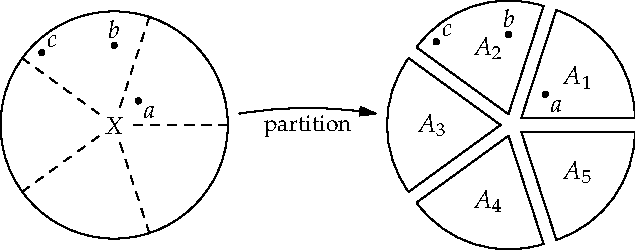
\includegraphics[width=0.7\textwidth]{relations-08-part}\\
	Each element of $X$ ends up in exactly one subset. In the language of the Theorem, we have\\[5pt]
	$A_1=[a]$,\quad $A_2=[b]=[c]$,\quad $b\sim c$,\quad $a\nsim b$, \quad $a\nsim c$.
\end{center}

Some things to consider while reading the proof:
\begin{itemize}
  \item Think about the picture! The result is nothing more than the notion of partitioning a cake by cutting it into slices. The slices are the equivalence classes of the obvious relation: two crumbs are related if and only if they lie in the same slice. The algebra that follows merely confirms that the picture is telling a legitimate story.
  \item In part 1.\ of the proof, look for where the reflexive, symmetric and transitive assumptions about $\sim$ are used. Why do we need $\sim$ to be an equivalence relation? Why does the proof fail if any of the three assumptions are dropped?
  \item Similarly, in part 2., look for where we use both parts of the definition of partition. Why are both assumptions required?
\end{itemize}



\begin{proof}
	\begin{enumerate}
		\item Assume that $\sim$ is an equivalence relation on $X$. To prove that the equivalence classes of $\sim$ partition $X$, we must show two things:
		\begin{enumerate}
	  	\item That every element of $X$ is in some equivalence class.
	  	\item That the distinct equivalence classes are pairwise disjoint: if $[x]\neq[y]$, then $[x]\cap[y]=\emptyset$.
		\end{enumerate}
		For (a), we only need reflexivity: $\forall x\in X$ we have $x\sim x$. Otherwise said, $x\in[x]$, whence every element of $X$ is in the equivalence class defined by itself.\par
		For (b), we prove by the contrapositive method and show that $[x]\cap [y]\neq\emptyset\implies [x]=[y]$.\par
		Assume that $[x]\cap [y]\neq\emptyset$. Then $\exists z\in [x]\cap [y]$. This gives
		\begin{align*}
			z\sim x\ \text{ and }\ z\sim y&\implies x\sim z\ \text{ and }\ z\sim y\tag*{(Symmetry)}\\*
			&\implies x\sim y\tag*{(Transitivity)}\\*
			&\implies [x]=[y]\tag*{(Lemma \ref{lemm:preequiv})}
		\end{align*}
		We have proved (b) and therefore part 1.\ of the theorem.
		\item Now suppose that $\{A_n:n\in I\}$ is a partition of $X$ and define $\sim$ by
		\[
			x\sim y\iff \exists n\in I\text{ such that $x\in A_n$ and $y\in A_n$.}
		\]
		We must prove the reflexivity, symmetry and transitivity of $\sim$.
		\begin{itemize}
			\item \refl Every $x\in X$ is in some $A_n$. Thus $x\sim x$ for all $x\in X$.
			\item \symm If $x\sim y$, then $\exists n\in I$ such that $x,y\in A_n$. But then $y,x\in A_n$ and so $y\sim x$.
			\item \trans Let $x\sim y$ and $y\sim z$. Then $\exists p,q\in I$ such that $x,y\in A_p$ and $y,z\in A_q$. Since $\{A_n:n\in I\}$ is a partition and $y\in A_p\cap A_q$, we necessarily have $A_p=A_q$. Thus $x,z\in A_p$ and so $x\sim z$.
		\end{itemize}
	
		We have shown $\sim$ is an equivalence relation, and the proof is complete.\qedhere
	\end{enumerate}
\end{proof}
	
Reading the proof carefully, you should see that reflexivity in part 2.\ comes from the fact that $X=\bigcup\limits_{n\in I}A_n$, while transitivity is due to the pairwise disjointness of the pieces of the partition. Symmetry is essentially free because the definition of $\sim$ is symmetric in $x$ and $y$.\par

The ability to partition sets and view the resulting subsets as individual objects is crucial to advanced mathematics. The importance of the Theorem comes from the fact that equivalence relations provide a straightforward \emph{algebraic} method of working with partitions.


\boldsubsubsection{Geometric Examples}

The language of equivalence relations and partitions is used heavily in geometry and topology to describe complex shapes. We finish this section with several examples. Since examples of partitions are especially easy to visualize with curves in the plane, we first return to the example on page \pageref{ex:equivcircle} and describe things in our new language.

\begin{example}{}{}
	For each real number $r\ge 0$, define the set\par
	\begin{minipage}[t]{0.63\linewidth}\vspace{0pt}
		\[
			A_r=\bigl\{(x,y)\in\R^2:x^2+y^2=r^2\bigr\}
		\]
		This is simply the circle of radius $r$ centered at the origin. We check that $\{A_r:r\in\R^+_0\}$ is a partition of $\R^2$.
		\begin{itemize}
	 		\item Every point of the plane lies on some circle. Precisely, $(x,y)\in A_{\sqrt{x^2+y^2}}$ since $\sqrt{x^2+y^2}$ is the distance of $(x,y)$ from the origin. Thus \smash{$\R^2=\bigcup\limits_{r\in\R^+_0}A_r$.}
	  	\item If $r_1\neq r_2$, then the concentric circles $A_{r_1}$ and $A_{r_2}$ do not intersect. Thus $A_{r_1}\cap A_{r_2}=\emptyset$.
		\end{itemize}
	\end{minipage}
	\hfill
	\begin{minipage}[t]{0.32\linewidth}\vspace{0pt}
		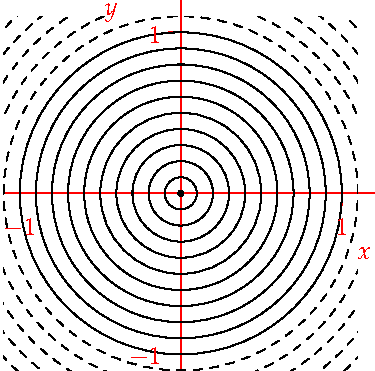
\includegraphics[width=\textwidth]{relations-09-circles}
	\end{minipage}\par

	Now define a relation $\sim$ on $\R^2$ via
	\[
		(x,y)\sim(v,w)\iff \exists r\ge 0\text{ such that $(x,y),(v,w)$ both lie on the circle $A_r$}
	\]
	By Theorem \ref{thm:equivpart} this is an equivalence relation. We can also check explicitly: dropping any mention of the radius $r$, we see that
	\[
		(x,y)\sim(v,w)\iff x^2+y^2=v^2+w^2
	\]
	This is exactly the equivalence relation described on page \pageref{ex:equivcircle}. The equivalence classes are precisely the sets $A_r$. Indeed for a given point $(v,w)$,
	\[
		[(v,w)]=\{(x,y)\in\R^2:x^2+y^2=v^2+w^2\}=A_{\sqrt{v^2+w^2}}
	\]
	is just the circle of radius $\sqrt{v^2+w^2}$.
\end{example}


\boldinline{The Möbius Strip}

Take a rectangle, for example $X=[0,6]\times[0,1]$, and partition into the following subsets.
\begin{itemize}
	\item If a point does not lie on the left or right edge of the rectangle, place it in a subset by itself: $\{(x,y)\}$ for $x\neq 0,6$,
	\item If a point does lie on the left or right edge of the rectangle, place it in a subset with one point from the other edge: $\{(0,y),(6,1-y)\}$ for any $y$.
\end{itemize}
The rectangle is drawn below, where the points on the left and right edges are colored red. The arrows indicate how the edges are paired up. For example the point $(0,0.8)$ (high on the left near the tip of the arrow) is paired with $(6,0.2)$ (low on the right edge of the rectangle).\par
These subsets clearly partition the rectangle $X$. The partitions define an equivalence relation $\sim$ on $X$ in accordance with Theorem \ref{thm:equivpart}. Note that there are infinitely many equivalence classes. The question is how we should interpret the quotient set $\quotient X\sim$?\par
This is easier to visualize than you might think. Since each point on the left edge of the rectangle lies in an equivalence class with a point on the right edge, we imagine gluing the two edges together in such a way that the corresponding points touch. In the picture, we imagine holding $X$ like a strip of paper, giving it a twist, and then gluing the edges together. This is the classic construction of a Möbius strip. The advantage of the quotient set calculation is that it is very easy to work with points in the original rectangle. As long as you permanently assume that equivalent points of the rectangle correspond to the same point of the Möbius strip you can easily work only in the rectangle.\par

\begin{center}
	\begin{tabular}{c}
		
\includegraphics[scale=3.4]{relations-10-mobius}\\
		Rectangle
	\end{tabular}
	\hspace*{.5cm}
	\begin{tabular}{c}
		
\includegraphics[scale=3.4]{relations-11-mobius}\\
		Half twist
	\end{tabular}\\[15pt]
	\begin{tabular}{c}
		
\includegraphics[width=0.65\textwidth,height=75pt]{relations-12-mobius}\\
		Glue arrows to obtain Möbius strip\\[15pt]
	\end{tabular}
\end{center}


% Let $L$ be the set of lines in the plane $\R^2$ and consider the relation $\ell_1\sim\ell_2\iff \ell_1$  is parallel to $\ell_2$. Then
% \begin{description}\itemsep=0pt
% \item[Reflexivity] $\ell\sim\ell$ since any line is parallel to itself.
% \item[Symmetry] $\ell_1\sim\ell_2\Rightarrow\ell_2\sim\ell_1$ since one line is parallel to a second iff the second is parallel to the first.
% \item[Transitivity] Suppose that $\ell_1$ is parallel to $\ell_2$, which is parallel to $\ell_3$, then $\ell_1$ is parallel to $\ell_3$; hence $\ell_1\sim \ell_2$ and $\ell_2\sim\ell_3\Rightarrow \ell_1\sim \ell_3$.
% \end{description}
% $\sim$ is therefore an equivalence relation. The equivalence class of a line is the set of all lines parallel to it: for example
% \[[y=2x-1]=\{y=2x+c:c\in\R\}.\]
% Each equivalence class is a copy of the real numbers. We can say more to get a handle on what the set of equivalence classes looks like. Every line in a fixed equivalence class has the same gradient $m\in\R\cup\{\infty\}$ (vertical, infinite gradient, lines are allowed!). To each $m\in\R\cup\{\infty\}$ there is exactly one equivalence class. In some sense you may therefore view $\{[\ell]\}=L/\sim$ as the set $\R\cup\{\infty\}$.\\
% Alternatively, all lines in an equivalence class make the same angle $\theta\in[0,180^\circ)$ with the $x$-axis. Replace each equivalence class by the point $(\cos 2\theta,\sin 2\theta)$ and we see that there is precisely one equivalence class for every point on the circle of radius one.\\
% We are tempted to say something like $L/\sim=\R\cup\{\infty\}=S^1$ (where $S^1$ is the circle). This is not correct, but the three sets are \emph{bijective} (we will see this in section \ref{sec:func}) and indeed \emph{homeomorphic}, which means topologically identical.

\boldinline{The Cylinder}%\label{page:cylinder}

We could construct a cylinder similarly to the Möbius strip, by identifying edges of the rectangle but \emph{without} applying the half-twist. Instead we do something a little different.\par

Let $X=\R^2$ with equivalence relation $\sim$ defined by
\[
	(a,b)\sim (c,d)\iff a-c\in\Z\quad\text{\emph{and}}\quad b=d
\]
The equivalence classes are horizontal strings of points with the same $y$ co-ordinate. If we imagine wrapping $\R^2$ repeatedly around a cylinder of circumference 1, all of the points in a given equivalence class will now line up. The set of equivalence classes $\quotient{\R^2}\sim$ can therefore be visualized as a cylinder.

Alternatively, you may imagine piercing a roll of toilet paper and unrolling it. The single puncture now becomes a row of (almost!\footnote{Unfortunately for the analogy, toilet paper has purposeful thickness!}) equally spaced holes.\par

In the picture, the left hand side is (part of) the plane $\R^2$, displayed so that points in each equivalence class have the same height and color. The three horizontal dots all lie in the same equivalence class. When we roll up the plane, all three points end up at the same point on the cylinder.

\begin{center}
	%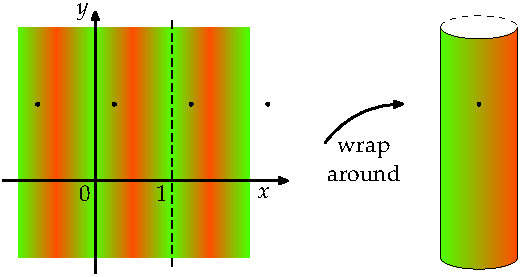
\includegraphics[scale=1.2]{relations-13-cylinder(mp)}\\
	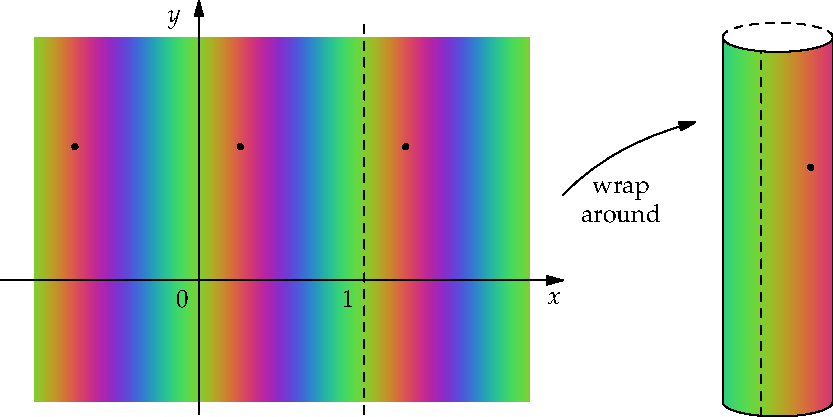
\includegraphics[width=0.8\textwidth]{relations-13-cylinder}
\end{center}

More complex shapes can be created by other partitions/relations. If you want a challenge in visualization, consider why the equivalence relation
\[
	(a,b)\sim (c,d)\iff a-c\in\Z\quad\text{\emph{and}}\quad b-d\in\Z
\]
on $\R^2$ defines a torus (the surface of a ring-doughnut).

% \paragraph{Self-test Questions}
% 
% \begin{enumerate}
%   \item What does it mean for a collection of subsets of a set $X$ to \emph{partition} $X$? You should be able to answer both using set notation and purely in a sentence.
%   \item True or false: if $X$ is partitioned into the equivalence classes of some equivalence relation $\sim$, then each element of $X$ lies in the equivalence class $[x]$.
%   \item True or false: Suppose that $X$ is partitioned into subsets and that $x,y,z\in X$. If $x,y$ lie in the same subset, and $y,z$ lie in the same subset of the partition, then it is possible for $x$ and $z$ to lie in different subsets.
%   \item Exhibit an infinite set $X$ and an equivalence relation $\sim$ on $X$ for which
%   \begin{enumerate}
%     \item $\quotient X\sim$ has finitely many elements.
%     \item $\quotient X\sim$ has infinitely many elements.
% 	\end{enumerate}
% \end{enumerate}


\begin{exercises}{}{}

\begin{enumerate}
	\item For each of the collections $\{A_n:n\in\R\}$, determine whether the collections partition $\R^2$. Justify your answers, and sketch several of the sets $A_n$.
	\begin{enumerate}
		\item $A_n=\big\{(x,y)\in\R^2:y=2x+n\big\}$.
	  \item $A_n=\big\{(x,y)\in\R^2:y=(x-n)^2\big\}$.
	  \item $A_n=\big\{(x,y)\in\R^2:xy=n\big\}$.
	  \item $A_n=\big\{(x,y)\in\R^2:y^4-y^2=x-n\big\}$.
	\end{enumerate}\pagebreak[2]
	
	\item Let $X$ be the set of all humans. If $x\in X$, we define the set
	\[A_x=\{\text{people who had the same breakfast \emph{or} lunch as $x$}\}.\]
	\begin{enumerate}
	  \item Does the collection $\{A_x:x\in X\}$ partition $X$? Explain your answer.
	  \item Is your answer different if the \emph{or} in the definition of $A_x$ is changed to \emph{and}?
	\end{enumerate}
	\emph{If Jane and Tom had both had the same breakfast and lunch, then $A_{\text{Jane}}=A_{\text{Tom}}$ so there are likely many fewer \emph{distinct} sets $A_x$ than there are humans!}
	
	\item Let $X=\{1,2,3\}$. Define the relation $\cR=\big\{(1,1),(1,2),(1,3),(2,1),(2,2),(3,1),(3,3)\big\}$ on $X$.
	\begin{enumerate}
	  \item Which of the properties reflexive, symmetric, transitive are satisfied by $\cR$?
	  \item Compute the sets $A_1,A_2,A_3$ where $A_n=\{x\in X:x\,\cR\,n\}$. Show that $\{A_1,A_2,A_3\}$ do not form a partition of $X$.
	  \item Repeat parts (a) and (b) for the relations $\cS$ and $\mathcal T$ on $X$, where
	  \begin{gather*}
	  \cS=\{(1,1),(1,3),(3,1),(3,3)\}\\
	  \mathcal T=\{(1,1),(1,2),(1,3),(2,1),(2,2),(2,3),(3,3)\}
	  \end{gather*}
	\end{enumerate}
	\emph{Some of the sets $A_1,A_2,A_3$ might be the same in each of your examples. If, for example, $A_1=A_3$, then the collection $\{A_1,A_2,A_3\}$ only contains two sets: $\{A_1,A_2\}$. Is this a partition? Compare with the example on page \pageref{ex:partnot}.}
  
	\item Using the equivalence relation description of the Möbius strip, prove that you may cut a Möbius strip round the middle and yet still end up with a single loop.\\
	\emph{Where would you cut the defining rectangle and how can you tell that you still have one piece?}

	
	\item (Hard!) A \emph{Klein bottle} can be visualized as follows. Define an equivalence relation $\sim$ on the unit square $X=[0,1]\times[0,1]$ so that:
	\begin{itemize}
	  \item $(0,y)\sim (1,y)$ for $0\le y\le 1$.
	  \item $(x,0)\sim(1-x,1)$ for $0\le x\le 1$.
	\end{itemize}
	The result is the picture: the blue edges are identified in the same direction and the red edges in the opposite. Attempting to visualize this in 3D requires a willingness to stretch and distort the square, but results in the green bottle. The original red and blue arrows have become curves on the bottle. If you are using Acrobat Reader, click on the bottle and move it around.
	\begin{enumerate}
	  \item Suppose you cut the Klein bottle along the horizontal dashed line of the defining square. What is the resulting object? What happens to the green bottle?
	  \item Now cut the square along the vertical dashed line. What do you get this time?
	\end{enumerate}
	Can you visualize where the two dashed lines are on the green bottle?
	
	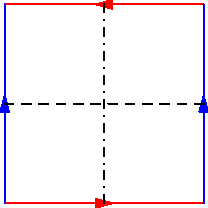
\includegraphics{relations-hw01-kleinsquare}
% 	\includemedia[width=0.99\textwidth, transparent=false, activate=onclick, add3Djscript=asylabels.js, %add3Djscript=3Dspintool.js,
% 3Dmenu,
%   3Dcoo=7.8239054679870605 -2.621169090270996 -71.13204956054688,
%   3Dc2c=-0.4364800751209259 0.7419548630714417 0.5089088082313538,
%   3Droo=219.44206346507434,
%   3Droll=-1.9382490979948275,
% 3Dlights=Headlamp]{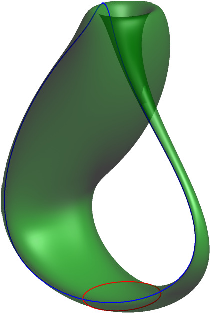
\includegraphics{relations-hw02-klein+0_0}}{relations-hw02-klein+0.prc}

\end{enumerate}

\end{exercises}

\clearpage


\subsection{Well-definition, Rings and Congruence}\label{sec:welldefn}

We return to our discussion of congruence (recall Section \ref{sec:cong}) in the context of equivalence relations and partitions. The important observation is that \emph{congruence modulo $n$ is an equivalence relation on $\Z$,} each equivalence class being the set of all integers sharing a remainder modulo $n$.

\begin{thm}{}{congequiv1}
	For a fixed $n\in\N$, define $x\sim_n y\iff x\equiv y\pmod n$. Then $\sim_n$ is an equivalence relation on $\Z$.
\end{thm}

The theorem is a restatement of Example \ref{ex:cong} on page \pageref{ex:cong}, in conjunction with Theorem \ref{thm:equivpart}. You should prove this yourself, as practice in using the definition of equivalence relation.\par
The equivalence classes are precisely those integers which are congruent modulo $n$: the integers which share the same remainder.
\begin{align*}
	[a]&=\big\{x\in\Z:x\equiv a\spmod n\big\}\\
	&=\big\{x\in\Z:x\text{ has the same remainder as $a$ when divided by $n$}\big\}\\
	&=\big\{x\in\Z:x-a\text{ is divisible by $n$}\big\}
\end{align*}
In this language, we can restate what it means for two equivalence classes to be equal.

\begin{thm}{}{congequiv2}
	$[a]=[b]\iff a\equiv b\pmod n\iff \exists k\in\Z\text{ such that }b=a+kn$.
\end{thm}

If the meaning of \emph{any} of the above is unclear, re-read the previous two sections: they are critically important!\par
The equivalence classes of $\sim_n$ partition the integers $\Z$. According to Theorem \ref{thm:congequiv2}, there are exactly $n$ equivalence classes, whence we may describe the quotient set as
\[
	\quotient \Z{\sim_n}=\big\{[0],[1],\ldots,[n-1]\big\}
\]
We use this set to define an extremely important object.

\begin{defn}{}{}
	Define operations $+_n$ and $\cdot_n$ on the set $\quotient\Z{\sim_n}$ as follows:
	\[
		[x]+_n[y]:=[x+y],\qquad [x]\cdot_n[y]:=[x\cdot y]
	\]
	The \emph{ring} $\Z_n$ is the set $\quotient\Z{\sim_n}$ together with the operations $+_n$ and $\cdot_n$.
\end{defn}

The operation $+_n$ is telling us how to add \emph{equivalence classes,} that is, how to produce a new equivalence class from two old ones. It is important to understand that $+_n$ is \emph{not the same} operation as $+$: we are \emph{defining} $+_n$ using $+$. The former combines equivalence classes, while the latter sums integers. The operation $\cdot_n$ similarly tells us how to multiply equivalence classes. The challenge here is that you have to think of each equivalence class as a single object. 

\begin{example}{}{}
	When we write
	\[
		[3]+_8[6]=[3+6]=[9]=[1]
	\]
	we are thinking about the equivalence classes $[3]$ and $[6]$ as individual objects rather than as collections of elements: remember that $[3]=\{\ldots,-5,3,11,19,\ldots\}$ is an infinite set! There is, moreover, a matter of choice: since, for example, $[3]=[11]$ and $[6]=[22]$ we should be able to observe that
	\[
		[3]+_8[6]=[11]+_8[22]
	\]
	Is this true? If not, then the operation $+_8$ would not be particularly useful. Thankfully this is not a problem: according to the definition of $+_8$, we have
	\[
		[11]+_8[22]=[11+22]=[33]=[1]
	\]
	exactly as we would wish.
\end{example}

Let us think a little more abstractly. Suppose we are given equivalence classes $X$ and $Y$, how do we compute $X+_nY$? Here is the process.
\begin{enumerate}
  \item \emph{Choose} elements $x\in X$ and $y\in Y$ so that $X=[x]$ and $Y=[y]$.
  \item Add $x$ and $y$ to get a new element $x+y\in\Z$.
  \item Then $X+_nY$ is the equivalence class $[x+y]$.
\end{enumerate}
The issue is that there are \emph{infinitely many possibilities} for the elements $x\in X$ and $y\in Y$ chosen at step 1. If $+_n$ is to make sense, we must obtain the \emph{same} equivalence class $[x+y]$ {\bf regardless of our choices of $x\in X$ and $y\in Y$.}

\begin{defn}{}{well}
	A concept is \emph{well-defined} if it is \emph{independent of all choices used in the definition.}
\end{defn}

\begin{thm}{}{congwd}
	The operations $+_n$ and $\cdot_n$ are well-defined.
\end{thm}

The choices made in the definitions of $+_n$ and $\cdot_n$ were of representative elements $x$ and $y$ of the equivalence classes $[x]$ and $[y]$. All representatives of these classes have the form
\[
	x+kn\in[x]\quad\text{and}\quad y+ln\in[y]
\]
for some integers $k,l$. It therefore suffices to prove that
\[
	\forall k,l\in\Z,\quad [x+kn]+_n[y+ln]=[x]+_n[y]\quad\text{and}\quad [x+kn]\cdot_n[y+ln]=[x]\cdot_n[y]
\]
We are now in a position to prove the Theorem.

\begin{proof}
	We prove that $+_n$ is well-defined.
	\begin{align*}
		[x+kn]+_n[y+ln]&=[(x+kn)+(y+ln)]\tag*{(by definition of $+_n$)}\\
		&=[x+y+(k+l)n]\\
		&=[x+y]\tag*{(by Theorem \ref{thm:congequiv2})}\\
		&=[x]+_n[y]\tag*{(by definition of $+_n$)}
	\end{align*}
	The argument for $\cdot_n$ is similar.
\end{proof}

You should re-read Theorem \ref{thm:congbasic} until you are comfortable that we are doing the same thing!

\begin{aside}{}{}
{\bf Aside: Ugly notation}

Given the usefulness of $\Z_n$ and the cumbersome nature of the above notation, it is customary to drop the square brackets and subscripts and simply write
\[
	\Z_n=\{0,1,2,\ldots,n-1\},\qquad x+y:=x+y\spmod n,\qquad x\cdot y:=xy\spmod n
\]
When using this description of $\Z_n$, you should realize that we are working with equivalence classes, not numbers. In this context, $-3\in\Z_8$ makes perfect sense, for it really means $[-3]\in\Z_8$. This is perfectly fine, since $[-3]=[5]$ as equivalence classes, whence it is legitimate to write $-3=5$ in $\Z_8$. Until you are 100\% sure that you know when 3 represents an equivalence class and when it represents a number, you should keep the brackets in place: in particular it might be a good idea to keep using them until you have passed \emph{this course}!
\end{aside}

% 
% \paragraph{Self-test Questions}
% 
% \begin{enumerate}
%   \item Which of the following are true and which false?
%   \begin{enumerate}
%     \item $[28]=[5]$ in $\Z_6$.
%     \item $[24]+\big([3]+[17]\big)=[-10]$ in $\Z_9$.
%     \item $[2]^3+[3]^3=[4]^3$ in $\Z_{29}$.
% 	\end{enumerate}
% 	\item Explain the difference between the operations $+,\cdot$ on $\Z_n$ and $+,\cdot$ on $\Z$. Is the following true or false?
% 	\[[x]+[y]=[z]\iff x+y=z.\]
% \end{enumerate}

\begin{exercises}{}{}

\begin{enumerate}
  \item\begin{enumerate}
    \item Explicitly check that $[7]+[21]=[98]+[-5]$ in $\Z_{13}$.
    \item Suppose that $[5]\cdot[7]=[8]\cdot[9]$ makes sense. Find the value of $n$ if we are working in the ring $\Z_n$.
  \end{enumerate}
  
  \item\begin{enumerate}
    \item Prove the second half of Theorem \ref{thm:congwd}, that $\cdot_n$ is well-defined.
	  \item Prove by induction that the operation of raising to the power $m\in\N$ is well-defined in $\Z_n$. I.e., prove that
  \[\forall m\in\N,\ \forall [x]\in\quotient{\Z}{\sim_n}\text{ we have } [x^m]=[x]^m.\]
  \emph{Be careful! $n$ is fixed, your induction variable is $m$. What base case(s) do you need?}
  \end{enumerate} 
  
  \item Give an explicit proof of Theorem \ref{thm:congequiv1}.
  
  \item\label{ex:qequiv} Consider the relation $\sim$ defined on $\Z\times\N=\{(x,y):x\in\Z,\text{ and }y\in\N\}$ by
  \[(a,b)\sim(c,d)\iff ad=bc.\]
  \begin{enumerate}
    \item Prove that $\sim$ is an equivalence relation.
    \item List several elements of the equivalence class of $(2,3)$. Repeat for the equivalence class of $(-3,7)$. What do the equivalence classes have to do with the set of rational numbers $\Q$?
    \item Define operations $\oplus$ and $\otimes$ on $\quotient{\Z\times\N}\sim$ by
    \[[(a,b)]\oplus[(c,d)]=[(ad+bc,bd)],\qquad [(a,b)]\otimes[(c,d)]=[(ac,bd)].\]
    Prove that $\oplus$ and $\otimes$ are well-defined.
  \end{enumerate}
  \emph{Try to do this question \emph{without} using division! We will return to this example in the next section.}
\end{enumerate}

\end{exercises}
\clearpage



\subsection{Functions and Partitions (Optional)}

To complete our discussion of partitions and equivalence relations, we consider how to define a function whose domain is a set of equivalence classes. We take congruence as our motivating example.\par

Suppose we want to define a function $f:\Z_4\to\Z_6$. Say $f(x)=3x\pmod 6$. This certainly looks like a function, but is it? Remember that `$x$' and `$3x$' are really equivalence classes, so we should say\footnote{The notation $[x]_4$ is helpful for reminding us which equivalence relation is being applied. When dealing with functions between different quotient sets, it is easy to become confused.}
\[
	f\bigl([x]_4\bigr)=[3x]_6,\qquad\text{where}\quad [x]_4\in\Z_4\quad\text{and}\quad [3x]_6\in\Z_6
\]
Is \emph{this} a function? To make sure, we need to check that \emph{any} representative $a\in[x]_4$ gives the same result. That is, we need to prove that
\[
	a\equiv b\spmod 4\implies 3a\equiv 3b\spmod 6
\]
This is not so hard:
\begin{align*}
	a\equiv b\spmod 4&\implies \exists n\in\Z\text{ such that }a=b+4n\\
	&\implies 3a=3b+12n\implies 3a\equiv 3b\spmod 6.
\end{align*}
It might appear to be a minor difference, but attempting to define $g:\Z_4\to\Z_6$ by $g(x)=2x\pmod 6$ does \emph{not} result in a function. If it were, then we should have
\[
	a\equiv b\spmod 4\implies 2a\equiv 2b\spmod 6
\]
But this is simply not true: for example $4\equiv 0\pmod 4$, but $8\not\equiv 0\pmod 6$. It might look like $g$ is a function, but it is not well-defined because $[4]=[0]$ in $\Z_4$ and $g\bigl([4]\bigr)\neq g\bigl([0]\bigr)$ in $\Z_6$.\par

Just as in Definition \ref{defn:well}, the process of verifying that a rule really is a function is called checking \emph{well-definition.} In general, if we are defining a function
\[
	f:\quotient X\sim\to A
\]
whose domain is a quotient set, then it is usually necessary to construct $f$ by saying what happens to a \emph{representative} $x$ of an equivalence class $[x]$:
\[
	f\bigl([x]\bigr)=\text{ `do something to $x$'.}\tag{$\ast$}
\]
We need to make sure that the `something' is \emph{independent of the choice of element} $x$.

\begin{defn}{}{}
	Suppose that $f:\quotient X\sim\to A$ is a rule of the form ($\ast$). We say that $f$ is a \emph{well-defined} function if
	\[
		[x]=[y]\implies f\bigl([x]\bigr)=f\bigl([y]\bigr)
	\]
\end{defn}

If you think carefully, this is nothing more than condition 2.\ of Definition \ref{defn:func}.

\begin{examples}{}{}
\begin{enumerate}
	\item Show that $f:\Z_n\to\Z_n$ defined by $f(x)=x^2+4\pmod n$ is well-defined.\par
	We must check that $x\equiv y\pmod n\implies x^2+4\equiv y^2+4\pmod n$. But this is trivial!
	\item For which integers $k$ is the rule $f_k:\Z_4\to\Z_6$ defined by $f_k(x)=kx\pmod 6$ a well-defined function?\par
	We start with a special case. If $k=1$, then we can attempt to construct a table of values for $f_1(x)$:
	\[
		\begin{array}{c|cccc|cccc|cc}
			x&0&1&2&3&4&5&6&7&8&\cdots\\\hline
			f_1(x)&0&1&2&3&4&5&0&1&2&\cdots
		\end{array}
	\]
	The problem is immediately visible! In $\Z_4$ we have $0=4$, however $f_1(0)=0$ and $f_1(4)=4$ \emph{which are not equal in $\Z_6$}! It follows that $f_1$ is not a function.\par
	Rather than try out all possible values of $k$, we proceed systematically. If $f_k$ is to be well-defined, we require $x\equiv y\pmod 4\implies kx\equiv ky\pmod 6$. Now
	\begin{align*}
		x\equiv y\pmod 4&\implies \exists n\in\Z\text{ such that }x-y=4n\\*
		&\implies kx-ky=4kn
	\end{align*}
	For $f_k$ to be well-defined, we need to see that $k(x-y)=4kn$ is a multiple of 6 \emph{independently} of $x$ and $y$. Thus $f_k$ is well-defined if and only if $6\mid 4kn$\, \emph{for all} $n\in\Z$. This is the case if and only if $6\mid 4k$. Otherwise said,
	\[
		\text{$f_k$ is well-defined}\iff 6\mid 4k\iff 3\mid 2k\iff 3\mid k
	\]
	Given that we want $kx\in\Z_6$, we need only consider $k\in\{0,1,2,3,4,5\}$: equivalent values of $k$ modulo 6 won't change the definition of $f_k$. It follows that there are only \emph{two} well-defined functions $f_k:\Z_4\to\Z_6:x\mapsto kx$, namely $f_0(x)=0$ and $f_3(x)=3x$. Here they are in tabular form.
	\[
		\begin{array}{c|cccc|cccc|cc}
			x&0&1&2&3&4&5&6&7&8&\cdots\\\hline
			f_0(x)&0&0&0&0&0&0&0&0&0&\cdots\\\hline
			f_3(x)&0&3&0&3&0&3&0&3&0&\cdots
		\end{array}
	\]
	It should be clear that well-defined functions $f_k$ produce tables whose $f_k(x)$ line is \emph{periodic with period four.} To ram this point home, here is the table when $k=5$:
	\[
		\begin{array}{c|cccc|cccc|cc}
			x&0&1&2&3&4&5&6&7&8&\cdots\\\hline
			f_5(x)&0&5&4&3&2&1&0&5&4&\cdots
		\end{array}
	\]
	This is palpably not a function! You should compare these examples with those on page \pageref{ex:functmod1} and with Exercise \ref*{sec:func1}.\ref{ex:kfunc}. Are these earlier example still functions when the domains are assumed to be a ring $\Z_n$ rather than simply a set of integers?
\end{enumerate}
\end{examples}


\boldsubsubsection{Functions on the Cylinder and Torus}%\label{subsec:cylinder}

Recall our construction on page \pageref{page:cylinder}, where we viewed the cylinder as the set $\quotient{\R^2}\sim$ with respect to the equivalence relation
\[
	(a,b)\sim (c,d)\iff a-c\in\Z\quad\text{and}\quad b=d
\]
We wish to define a function $f$ whose domain is a cylinder. Using the equivalence relation, this is the same as defining a function $f:\quotient{\R^2}\sim\to A$ where $A$ is our chosen codomain. \emph{Well-definition} requires that $f$ satisfy
\[
	(a,b)\sim(c,d)\implies \smash{f\Bigl(\bigl[(a,b)\bigr]\Bigr)=f\Bigl(\bigl[(c,d)\bigr]\Bigr)}
\]
Since $(a,b)\sim(a+1,b)$, we require $f\Bigl(\bigl[(a,b)\bigr]\Bigr)=f\Bigl(\bigl[(a+1,b)\bigr]\Bigr)$, for all $a,b\in\R$.
Otherwise said, $f\Bigl(\bigl[(x,y)\bigr]\Bigr)$ must be periodic in $x$ with period one. It is easy to see that
\[
	\smash{f\Bigl(\bigl[(x,y)\bigr]\Bigr)=y^2\sin(2\pi x)}
\]
is a suitable choice of function $f:\quotient{\R^2}\sim\to\R$.\par

More generally, to define a function whose domain is the torus
\[
	T^2=\quotient{\R^2}\sim\quad\text{where}\quad (a,b)\sim (c,d)\iff a-c\in\Z\quad\text{and}\quad b-d\in\Z
\]
requires a function which is periodic in \emph{both} $x$ and $y$. The function
\[
	f\Bigl(\bigl[(x,y)\bigr]\Bigr)=\sin(2\pi x)\cos(2\pi y)
\]
is plotted below, with the color on the torus indicating the value of $f$. It is easier to instead consider the function
\[
	F:\R^2\to\R:(x,y)\mapsto\sin(2\pi x)\cos(2\pi y)
\]
This is also plotted, with the same color for each value. The point is that $F$ is really $f$ in disguise, but has the advantage of being much easier to work with.

% \begin{center}
% 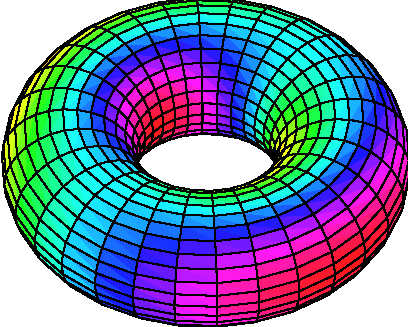
\includegraphics[scale=1]{relations-14-torus(maple)}\\
% The function $f$: domain $T^2$\\[.2cm]
% 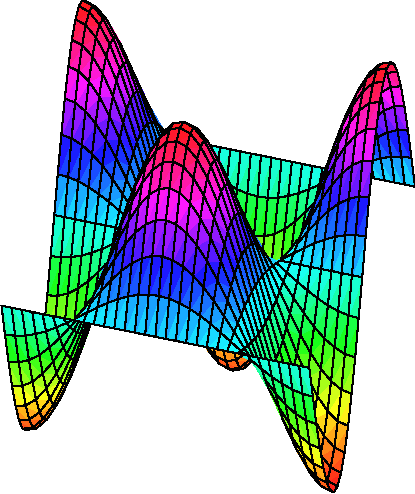
\includegraphics[scale=.6]{relations-15-plane}\quad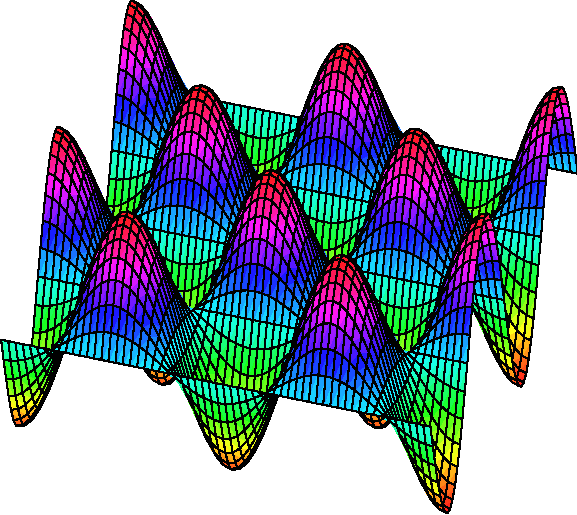
\includegraphics[scale=.6]{relations-16-plane2}\\
% The function $F$: domains $0\le x,y\le 1$ and $0\le x,y\le 2$ respectively
% \end{center}

\begin{center}
	\begin{minipage}{0.45\textwidth}\centering
		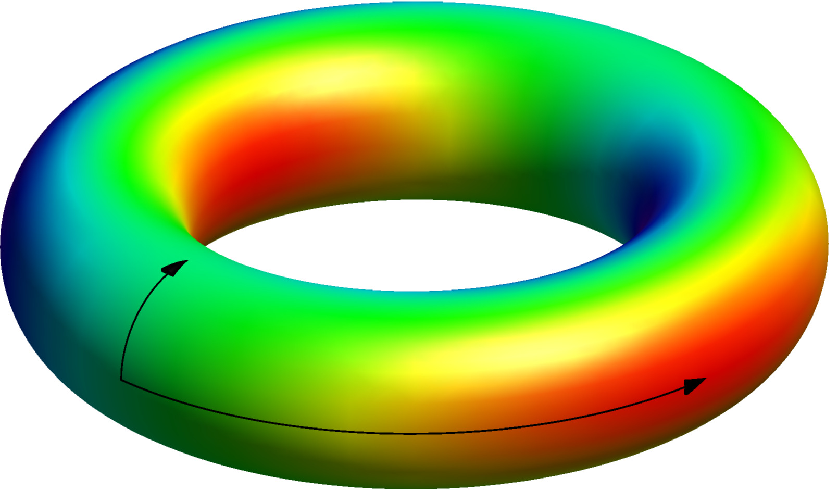
\includegraphics[width=\textwidth]{relations-14-torus}\\[14pt]
		The function $f$: domain $T^2$\\
		The arrows in the two pictures correspond
	\end{minipage}\qquad
	\begin{minipage}{0.45\textwidth}\centering
		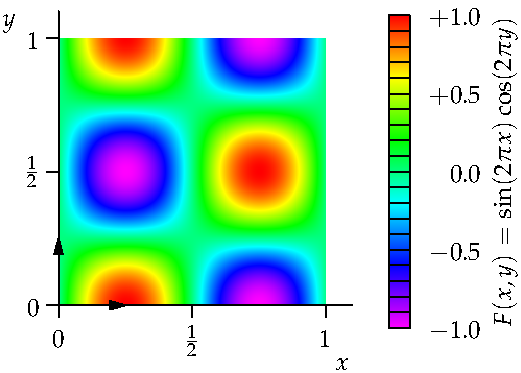
\includegraphics[width=\textwidth]{relations-14-torus2}\\
		The function $F$ restricted to $[0,1)\times [0,1)$
	\end{minipage}
\end{center}

\boldsubsubsection{Optional: The Canonical Map}

To do this justice, and to give you a taste for the details which are necessary in pure mathematics, here is the important definition.

\begin{defn}{}{}
	Suppose that $\sim$ is an equivalence relation on a set $X$. The function $\gamma:X\to \quotient X\sim$ defined by $\gamma(x)=[x]$ is the \emph{canonical map.}\footnote{Canonical, in mathematics, just means natural or obvious.}
\end{defn}

For us, the purpose of the canonical map is to allow us to construct functions $f:\quotient X\sim\to A$.

\begin{thm}{}{}
	Suppose that $\sim$ is an equivalence relation on $X$.
	\begin{enumerate}
  	\item If $f:\quotient X\sim\to A$ is a function, then $F:X\to A$ defined by $F=f\circ\gamma$ satisfies
  	\[
  		x\sim y\implies F(x)=F(y)
  	\]
  	\item If $F:X\to A$ satisfies $x\sim y\implies F(x)=F(y)$, then there is a unique function $f:\quotient X\sim\to A$ satisfying $F=f\circ\gamma$.
	\end{enumerate}
\end{thm}

\begin{proof}
\begin{enumerate}
  \item\begin{align*}
	\hspace{4.3pt}\text{This is trivial:}\quad x\sim y&\implies [x]=[y]\implies \gamma(x)=\gamma(y)\\
	&\implies f(\gamma(x))=f(\gamma(y))\implies F(x)=F(y).
	\end{align*}\
	\item $f:\quotient X\sim\to A$ can only be the function \emph{defined} by $f([x])=F(x)$. We show that this is well-defined:
	\begin{gather*}
	[x]=[y]\implies x\sim y\implies F(x)=F(y)\implies f([x])=f([y]).\tag*{\qedhere}
	\end{gather*}
\end{enumerate}
\end{proof}

\begin{minipage}[t]{0.65\linewidth}\vspace{0pt}
	The proof, like much of mathematics, is a masterpiece in concision that seems to be doing nothing at all. The point is that functions of the form $f:\quotient X\sim\to A$ are \emph{difficult} to work with. The Theorem says that we never need to explicitly use such functions, and can instead work with \emph{simpler} functions of the form $F:X\to A$. The only condition is that we must have $x\sim y\implies F(x)=F(y)$. Essentially, $F$ is $f$ in disguise!
\end{minipage}
\hfill
\begin{minipage}[t]{0.3\linewidth}\vspace{0pt}
	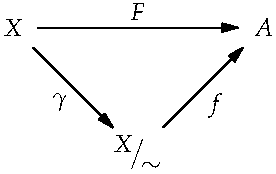
\includegraphics[width=\textwidth]{relations-17-isomthm}
\end{minipage}\par

This result will be resurrected when you study Groups, Rings \& Fields as part of the famous \emph{First Isomorphism Theorem.}


% \paragraph{Self-test Questions}
% 
% \begin{enumerate}
%   \item Let $k$ be a constant integer. If $f:\Z_5\to\Z_{18}:x\mapsto kx$ is a well-defined function, what period must the sequence of values $f(0),f(1),f(2),\ldots$ have?
%   \item State what it means for a function $f:\quotient X\sim\to A$ to be well-defined.
% \end{enumerate}

\begin{exercises}{}{}
\begin{enumerate}
	\item\begin{enumerate}
	  	\item Prove or disprove: $f:\Z_3\to\Z_5:x\mapsto x^3\pmod 5$ is well-defined.
			\item Prove or disprove: $f:\Z_{10}\to\Z_{20}:x\mapsto x^2\pmod{20}$ is well-defined.
		\end{enumerate}
		
	\item Can we view $F(x,y)=(y^2-1)\sin^2(\pi x)$ as a function whose domain is the cylinder, as described on page \pageref{subsec:cylinder}? Explain your answer. 

	\item\begin{enumerate}
	  	\item Compute $(x+4n)^2$.
	  	\item Suppose that $\forall n\in\Z$, we have $(x+4n)^2\equiv x^2\pmod m$. Find all the integers $m$ for which this is a true statement.
	  	\item For what $m\in\N_{\ge 2}$ is the function $f:\Z_4\to\Z_m:x\mapsto x^2\pmod m$ well-defined.
		\end{enumerate}
		
	\item A rule $f:\quotient X\sim\to A$ is well-defined if $[x]=[y]\implies f\bigl([x]\bigr)=f\bigl([y]\bigr)$.
	\begin{enumerate}
	  \item State what it means for $f:\quotient X\sim\to A$ to be \emph{injective.} What do you observe?
	  \item Prove that $f:\Z_7\to\Z_{35}:x\mapsto 15x$ is a well-defined, injective function.
	  \item Repeat part (b) for the function $f:\Z_{100}\to\Z_{300}:x\mapsto 9x$. Compare your arguments for well-definition and injectivity.\\
	  \emph{This forces you to write your argument abstractly, rather than using a table! You may find it useful that $9\cdot(-11)\equiv 1\pmod{100}$.}
	\end{enumerate}

	\item Define a partition of the sphere $S^2=\bigl\{(x,y,z):x^2+y^2+z^2=1\bigr\}$ into subsets of the form
	\[\bigl\{(x,y,z),(-x,-y,-z)\bigr\}.\]
	Each subset consists of two points directly opposite each other on the sphere (antipodal points). Let $\sim$ be the equivalence relation whose equivalence classes are the above subsets.
		\begin{enumerate}
	  	\item $f:\quotient{S^2}{\sim}\to\R:[(x,y,z)]\mapsto xyz$ is not well-defined. Explain why.
	  	\item Prove that $f:\quotient{S^2}{\sim}\to\R^3:[(x,y,z)]\to(yz,xz,xy)$ is a well-defined function.\\
			\emph{The image of this function is Steiner's famous \href{http://en.wikipedia.org/wiki/Roman_surface}{Roman Surface}, another example, like the Klein Bottle, of a generalization of the M\"obius Strip.}
		\end{enumerate}
		
		\item Recall Exercise \ref*{sec:welldefn}.\ref{ex:qequiv}, where we defined an equivalence relation $\sim$ on $\Z\times\N$.
		\begin{enumerate}
			\item	Prove that the function $f:\quotient{\Z\times\N}\sim\to\Q$ defined by $f\Bigl(\bigl[(x,y)\bigr]\Bigr)=\frac xy$ is a \emph{well-defined bijection.}
			\item Prove that $f$ transforms the operations $\oplus$ and $\otimes$ into the usual addition and multiplication of rational numbers. That is:
			\begin{gather*}
			f\Bigl(\bigl[(a,b)\bigr]\oplus\bigl[(c,d)\bigr]\Bigr)=f\Bigl(\bigl[(a,b)\bigr]\Bigr)+f\Bigl(\bigl[(c,d)\bigr]\Bigr)\\
			f\Bigl(\bigl[(a,b)\bigr]\otimes\bigl[(c,d)\bigr]\Bigr)=f\Bigl(\bigl[(a,b)\bigr]\Bigr)\cdot f\Bigl(\bigl[(c,d)\bigr]\Bigr)
			\end{gather*}
			\emph{The technical term for this is that $f:\left(\quotient{\Z\times\N}\sim,\oplus,\otimes\right)\to(\Q,+,\cdot)$ is an isomorphism of rings.}
		\end{enumerate}
\end{enumerate}

\end{exercises}

